\pdfminorversion=5 % to make it compatible with impressive
\documentclass[10pt]{beamer} % add gray to options to make it B&W

\def\myauthor{Adrià Arrufat}
\def\mytitle{Multiple transforms for video coding}
\def\myinstitute{Orange Labs and IETR/INSA --- Rennes, France}
\def\mydate{11th December 2015}

\usetheme{Berlin} % Antibes is also a nice theme
\usecolortheme{lily}
\usefonttheme{professionalfonts}
% \setbeamercolor{frametitle}{fg=black}
% \beamertemplateballitem
\definecolor{blueish}{RGB}{51,51,179}
\setbeamercolor{alerted text}{fg=blueish}
% \setbeamertemplate{footline}[frame number]
% add the frame number without destroying the template
\expandafter\def\expandafter\insertshorttitle\expandafter{%
  \insertshorttitle\hfill%
  \insertframenumber\,/\,\inserttotalframenumber\hfill\mydate}
\beamertemplatenavigationsymbolsempty % remove bottom naviation bar

\title{\mytitle}
\author{\myauthor}
\institute{\myinstitute}
\date{\mydate \\
	{\footnotesize Director: Olivier Déforges}\\
	{\footnotesize Supervisor: Pierrick Philippe}\\
	École Doctorale Matisse
}

\usepackage[T1]{fontenc}
% \usepackage{mathptmx}
\usepackage[scaled]{helvet}
\usepackage{courier}
\usepackage[helvet]{sfmath}
\usepackage{MnSymbol} % for the \curvearrowupdown symbol
\usepackage{nameref} % get section name
\usepackage{subfig}
\usepackage{ifthen}
\usepackage{siunitx} % consistent units and number support
\usepackage{multirow}
\usepackage{diagbox}
\usepackage{subfig} % subfloat environment
\makeatletter
\newcommand*{\currentname}{\@currentlabelname}
\makeatother

\usepackage{pgfplots,tikz}
\pgfplotsset{compat=1.12}
\usetikzlibrary{shapes,arrows,fit,calc,decorations.markings,intersections}
\usepgfplotslibrary{fillbetween}

\hypersetup{
	unicode=true,
	pdfencoding=auto,
	pdfauthor={\myauthor},
	pdftitle={\mytitle},
	pdfsubject={video coding},
	pdfkeywords={coding, image, video, transform},
	pdfinfo={
		CreationDate={D:20151017143523},
		%ModDate={...}
	},
}

\AtBeginSection[]
{%
	\frame<handout:0>
	{%
		\frametitle{Outline}
		\tableofcontents[currentsection,hideallsubsections]
	}
}

% custom definitions
\def\x{\mathbf{x}}
\def\X{\mathbf{X}}
\def\c{\mathbf{c}}
\def\A{\mathbf{A}}
\def\D{\mathbf{D}}
\def\Y{\mathbf{Y}}
\def\U{\mathbf{U}}
\def\V{\mathbf{V}}
\def\I{\mathbf{I}}
\def\P{\mathbf{P}}
\def\C{\mathbf{C}}
\def\y{\mathbf{y}}
\def\a{\mathbf{a}}
\def\L{\boldsymbol{\Lambda}}

\usebackgroundtemplate{%
\begin{tikzpicture}[remember picture, overlay]%
	\node at (current page.center) {
\includegraphics[width=0.9\paperwidth]{background}};%
\end{tikzpicture}}

\begin{document}

\maketitle

\usebackgroundtemplate{}
\section{General introduction}
\subsection{Context}
\begin{frame}{Era of the Internet and videos}
	\only<1>{
	\begin{block}{Current situation}
		\begin{itemize}
			\item In 2014: around 70\% of Internet traffic was due to video
				streaming
			\item Forecast for 2019: more than 80\%\footnote{Cisco Visual
				Networking Index: Forecast and Methodology, 2014--2019 White
				Paper}
		\end{itemize}
	\end{block}
	\begin{minipage}{0.49\textwidth}
		\begin{block}{Continuous need for video compression}
			\begin{itemize}
				\item {\bf New formats} emerge
				\item New applications require {\bf improved video quality}
				\item Need to decrease the bit-rate to stream/store videos
			\end{itemize}
		\end{block}
	\end{minipage}
	\begin{minipage}{0.49\textwidth}
		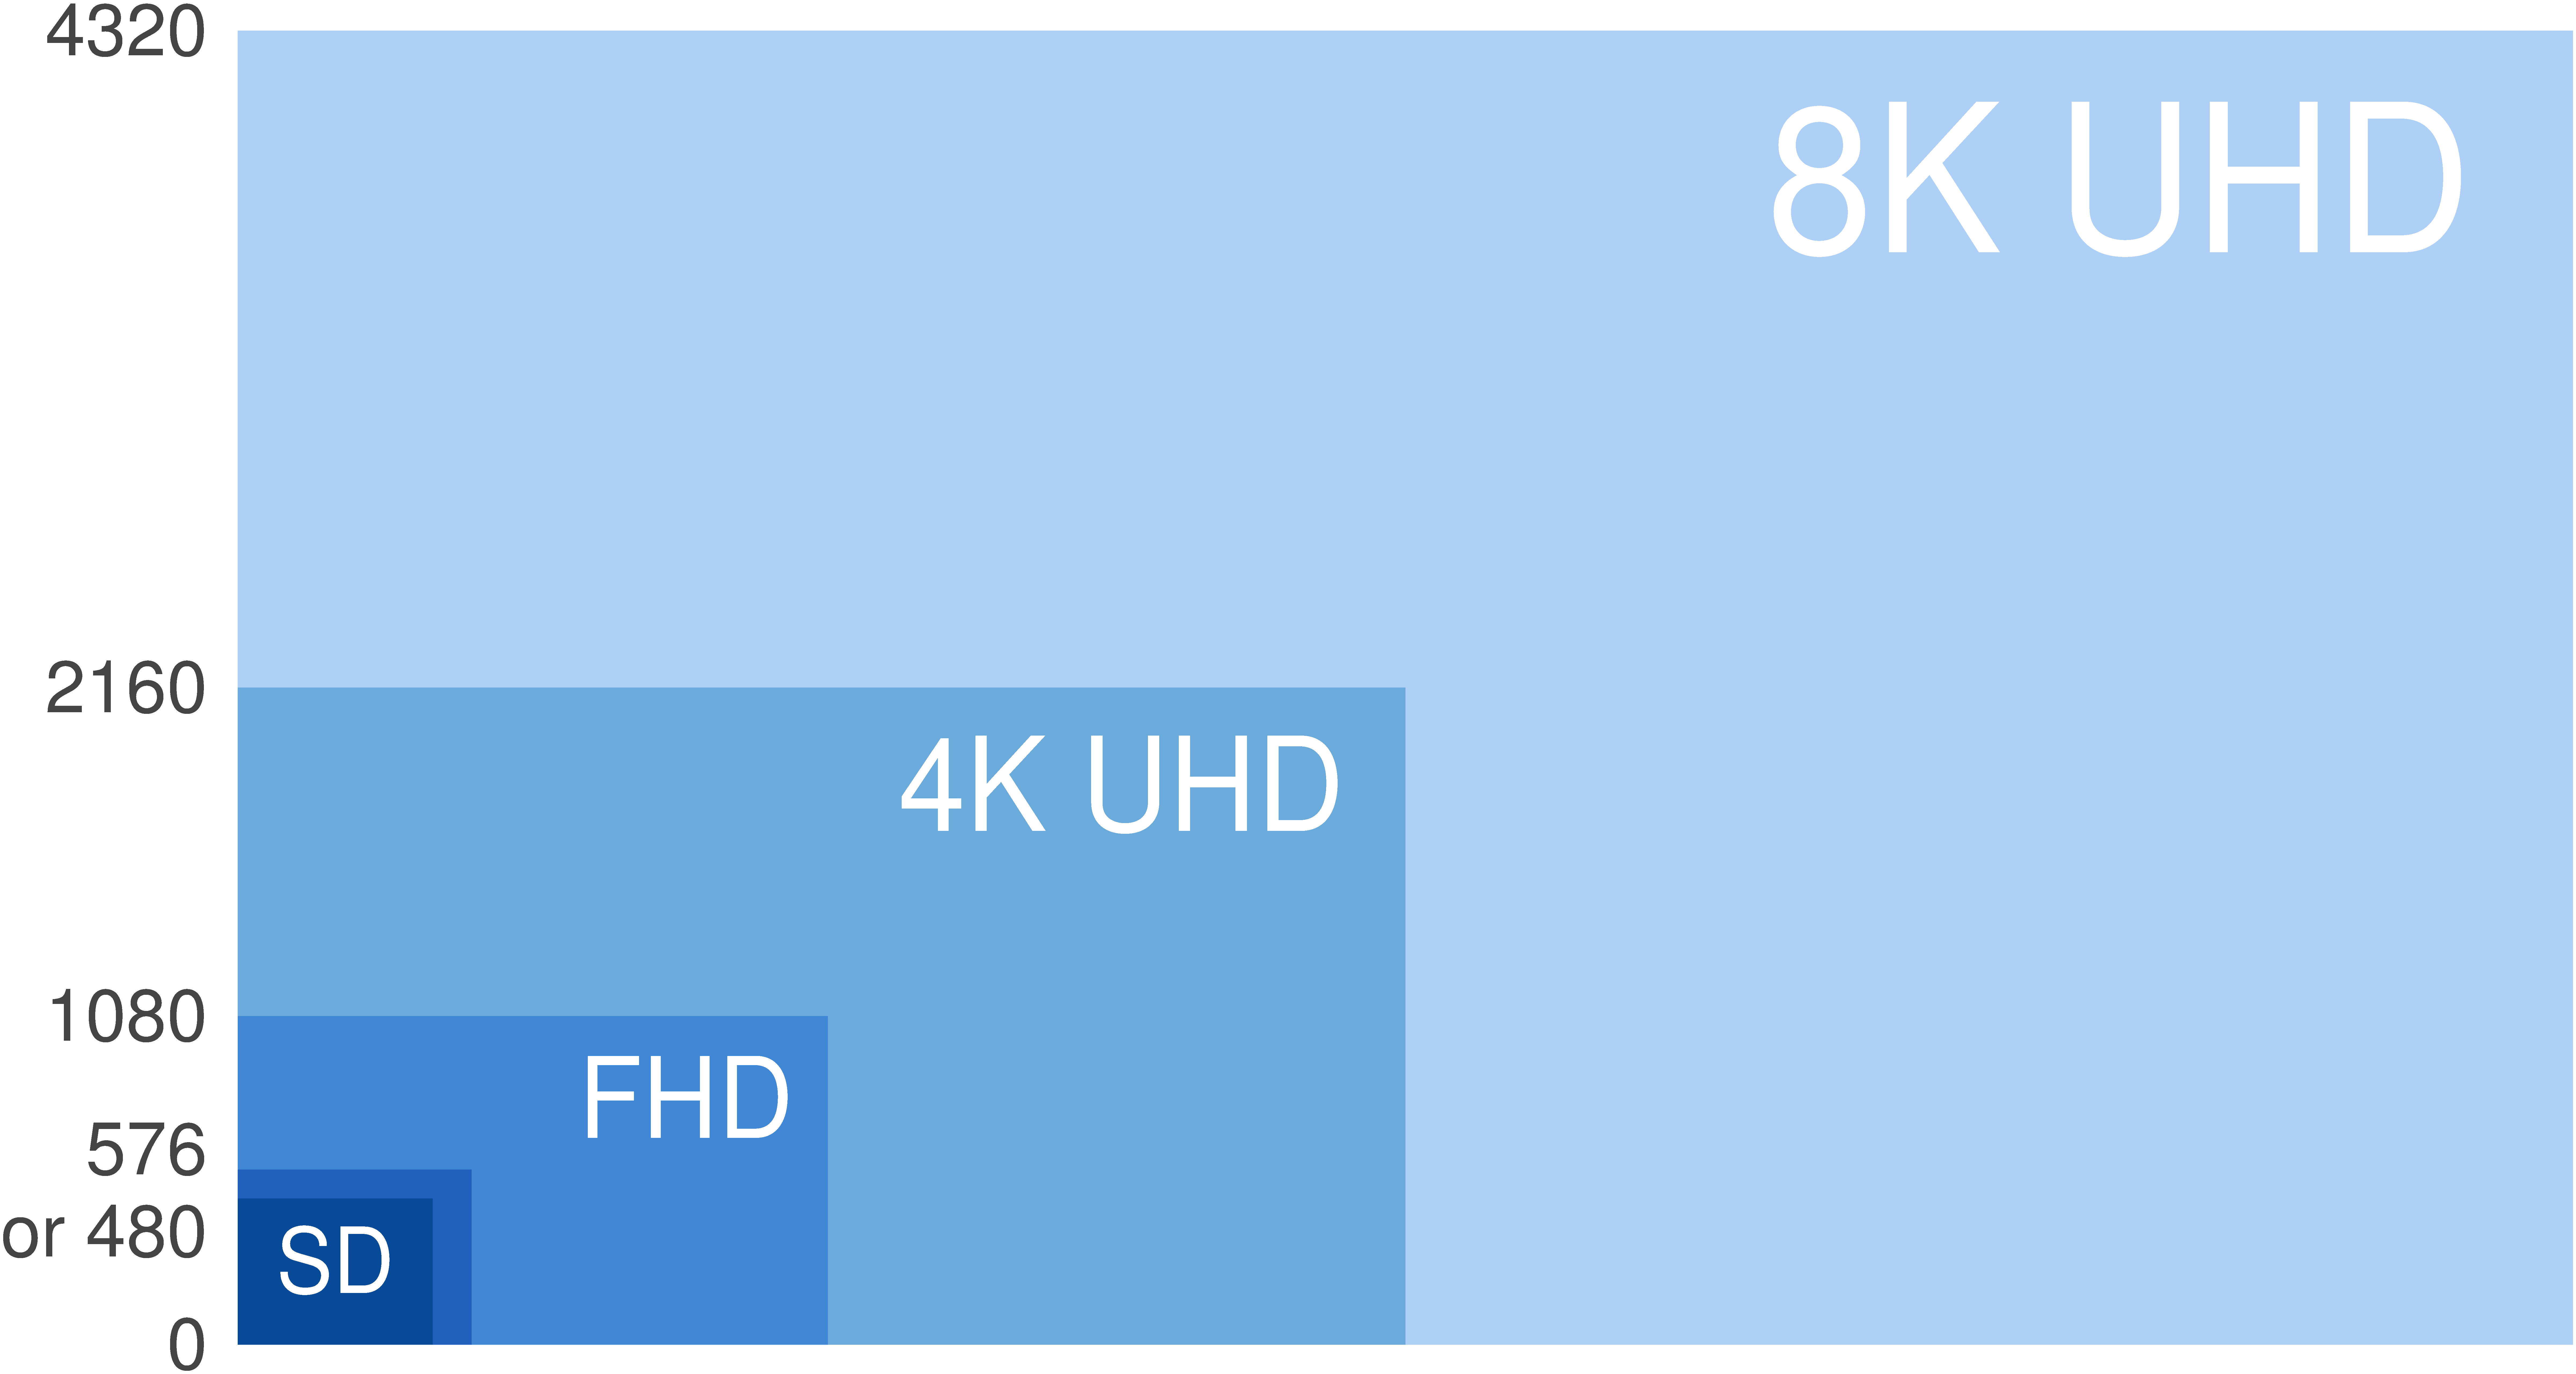
\includegraphics[width=\textwidth]{./figures/8K_UHD,_4K_SHD,_FHD_and_SD.eps}
	\end{minipage}
	}
	\only<2>
	{
	\begin{tikzpicture}
	\pgfplotsset{/tikz/font={\small}}
	\begin{axis}[
		grid=both,
		width=0.95\textwidth,
		height=0.95\textheight,
		x tick label style={
		/pgf/number format/1000 sep=},
		% scaled y ticks = false,
		% y tick label style={
		% 	/pgf/number format/.cd,
		% 	fixed,
		% 	set thousands separator={\thinspace},
		% 	fixed zerofill,
		% 	precision=0,
		% },
		ymax=100, ymin=0,
		ytick={0,20,...,100},
		ylabel={PB per month},
		enlarge y limits=false,
		enlarge x limits=0.04,
		legend pos=north west,
		legend cell align=left,
		ybar interval,
		xtick=data,
		xtick align=inside,
		]

		\addlegendentry{Internet video}
		\addplot coordinates {
		(2014, 21.624)
		(2015, 27.466)
		(2016, 36.456)
		(2017, 49.068)
		(2018, 66.179)
		(2019, 89.319)
		(2020, 0) % this line needs to be added so that it plots the previous one
		};

		\addlegendentry{Web, email, and data}
		\addplot coordinates {
		(2014,  5.853)
		(2015,  7.694)
		(2016,  9.476)
		(2017, 11.707)
		(2018, 14.002)
		(2019, 16.092)
		(2020, 0) % this line needs to be added so that it plots the previous one
		};

		\addlegendentry{File sharing}
		\addplot coordinates {
		(2014, 6.090)
		(2015, 6.146)
		(2016, 6.130)
		(2017, 6.168)
		(2018, 6.231)
		(2019, 6.038)
		(2020, 0) % this line needs to be added so that it plots the previous one
		};

		\addlegendentry{Online gaming}
		\addplot coordinates {
		(2014, 0.027)
		(2015, 0.033)
		(2016, 0.048)
		(2017, 0.078)
		(2018, 0.109)
		(2019, 0.143)
		(2020, 0) % this line needs to be added so that it plots the previous one
		};
	\end{axis}
\end{tikzpicture}

	}
\end{frame}

\begin{frame}{Standardisation}
	\begin{block}{Video coding standards}
		\begin{itemize}
			\item The work is inscribed inside a standardisation context
			\item Latest standard, HEVC, was released in 2013
		\end{itemize}
	\end{block}
	\begin{block}{Working context}
		\begin{itemize}
			\item Beginning of the standardisation phase
			\item Exploratory phase with relaxed complexity constraints
			\item Goal: achieve a suitable solution for a video coding
				standard for around 2020.
		\end{itemize}
	\end{block}
	\centering
	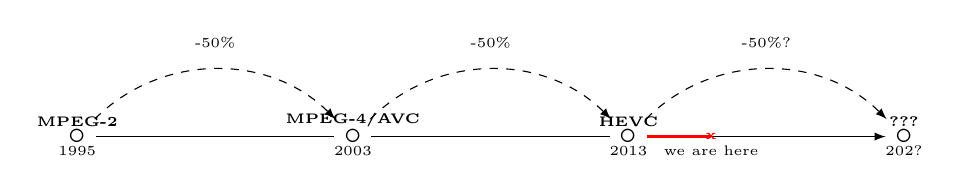
\begin{tikzpicture}[scale=1]
	\def\spacing{3.5}

	\node (mpeg2) at (0,0) {\scalebox{1.25}{$\circ$}};
	\node[above] at (mpeg2) {\tiny \bf MPEG-2};
	\node[below] at (mpeg2) {\tiny 1995};

	\node (mpeg4) at (\spacing,0) {\scalebox{1.25}{$\circ$}};
	\node[above] at (mpeg4) {\tiny \bf MPEG-4/AVC};
	\node[below] at (mpeg4) {\tiny 2003};

	\node (hevc) at (2*\spacing,0) {\scalebox{1.25}{$\circ$}};
	\node[above] at (hevc) {\tiny \bf HEVC};
	\node[below] at (hevc) {\tiny 2013};

	\node (???) at (3*\spacing,0) {\scalebox{1.25}{$\circ$}};
	\node[above] at (???) {\tiny \bf ???};
	\node[below] at (???) {\tiny 202?};

	\draw [-latex] (mpeg2) -- (mpeg4) -- (hevc) -- (???);

	\draw [dashed, -latex] (mpeg2) to [in=135, out=45] (mpeg4);
	\draw [dashed, -latex] (mpeg4) to [in=135, out=45] (hevc);
	\draw [dashed, -latex] (hevc) to [in=135, out=45] (???);

	\node [above] at (\spacing/2,1) {\tiny -50\%};
	\node [above] at (3*\spacing/2,1) {\tiny -50\%};
	\node [above] at (5*\spacing/2,1) {\tiny -50\%?};

	\node[red] (here) at (2.3*\spacing,0) {\tiny \bf x};
	\node[below] at (here) {\tiny we are here};
	\draw [thick,red] (hevc) --++ (3*\spacing/10,0);
\end{tikzpicture}

\end{frame}

\subsection{Video coding fundamentals}

\begin{frame}{The hybrid video coding scheme}
	\framesubtitle{Used in most video coding standards}
	\only<1>{\input{./figures/simp_hybrid_video_coding_scheme_1.tex}}
	\only<2>{\pgfmathsetmacro{\nodebasesize}{1} % A node with a value of one will have this diameter
\pgfmathsetmacro{\nodeinnersep}{0.1}

\newcommand{\propnode}[5]{% position, name, options, value, label
	\pgfmathsetmacro{\minimalwidth}{sqrt (#4*\nodebasesize)}
	\node[#3,minimum width=\minimalwidth*1cm,inner sep=\nodeinnersep*0cm,circle,draw] 
	(#2) at (#1) {#5};
}

\tikzstyle{bloq} = [rectangle, draw, text badly centered, minimum height=1em, inner sep=1mm]
\newcommand{\bloq}[4]{% position, name options, label
	\node[bloq,#3] (#2) at (#1) {\tiny\textsf{#4}}; 
}
\newcommand{\add}[2]{%position, name
	\draw (4,4) circle [radius=0.3] node (add) {\tiny\textsfi$+$};
}

\tikzstyle{frame} =
[rectangle, fill=white, draw, text centered, minimum width=4em, minimum height=2em]

\begin{tikzpicture}[scale=1.2,x=1em,y=1em]

% INPUT VIDEO SEQUENCE
	\draw (-2.35,0) node[above] {\tiny \textsf{Input Video Sequence}};
	\draw (-2,-3) node[above] {\tiny \textsf{Split into blocks}};
	\draw (-2,-3.5) node[above] {\tiny \textsf{Quad-tree partitioning}};
	\node[frame] at (-2.3,-0.7){};
	\node[frame] at (-2.2,-0.8){};
	\node[frame] at (-2.1,-0.9){};
	\node[frame] (sequence) at (-2,-1){};
	% \draw (-2,-1) --++ (0,0.85);
	% \draw (-2,-1) --++ (0,-0.85);
	% \draw (-2,-1) --++ (3.85,0);
	% \draw (-2,-1) --++ (-1.65,0);

	\filldraw[fill=blue!20, draw=blue!50,dashed,thick] 
	(1.5,-2) -- (15,-2) -- (15,-11.2) -- (1.5,-11.2) -- cycle;
	\node[below right] at (2,-2) {\tiny\textsf{Decoder}};
	\node[] at (2.75,-10.75) {\tiny\textsf{Intra/Inter}};

	\propnode{2,-1}{add1}{fill=green!50}{0}{\tiny$+$}
	\propnode{12,-6.5}{add2}{fill=green!50}{0}{\tiny$+$}
	\propnode{0.75,-1}{inter1}{fill=black}{0.005}{}
	\propnode{2,-6.5}{inter2}{fill=black}{0.005}{}
	\propnode{2,-8.75}{inter3}{fill=black}{0.005}{}
	\propnode{3.5,-7.5}{inter4}{fill=black}{0.005}{}
	\propnode{3.5,-10}{inter5}{}{0.005}{}
	\propnode{12,-1}{inter7}{fill=black}{0.005}{}
	\propnode{12.4,-6.5}{inter8}{fill=black}{0.005}{}
	\propnode{8.5,-8.75}{inter9}{fill=black}{0.005}{}

	\draw (add1) node[above] {\tiny\textsf{\hspace{3em}residuals}};

	\bloq{6,-1}{Transf}{text width=2.5em,fill=red!50}{Transform};
	\bloq{10,-1}{Quant}{text width=2em,fill=yellow!50}{Quant.};
	\bloq{6,-7.5}{IntraPred}{text width=2.5em,fill=yellow!50}{Intraframe\\[-1em]Prediction};
	\bloq{12,-3}{InvQuant}{text width=3.5em,fill=yellow!50}{Inv. Quant.};
	\bloq{12,-4.75}{InvTransf}{text width=3.5em,fill=red!50}{Inv. Transform};
	\bloq{6,-10}{MotionComp}{text width=2.5em,fill=yellow!50}{Motion\\[-1em]Est./Comp.};
	\bloq{19,-6.5}{EntrCod}{text width=2.5em,fill=yellow!50}{Entropy\\[-1em]Coding};
	\bloq{12,-8.75}{Reconst}{text width=3.2em,fill=white}{Reconst.\\[-0.5em]image};

	\draw[-latex,thick] (sequence) -- (add1) node [below right] {\tiny\textsf{$-$}};
	\draw[-latex,thick] (add1) -- (Transf);
	\draw[-latex,thick] (Transf) -- (Quant);
	\draw[-latex,thick] (InvQuant) -- (InvTransf);
	\draw[-latex,thick] (InvTransf) -- (add2);
	\draw[-latex,thick] (add2) -- (Reconst);
	\draw[-latex,thick] (inter2) -- (add2);
	\draw[-latex,thick] (inter3) -- (add1);
	\draw[-latex,thick] (IntraPred) -- (inter4);
	\draw[-latex,thick] (MotionComp) -- (inter5);
	\draw[thick] (inter3) -- (inter4);
	\draw[dotted,help lines, thick] (inter3) -- (inter5);
	%\draw[dotted,thin] (inter3) --++ (-40:1em) arc (-40:40:1em);
	\draw[-latex,thick] (Reconst) --++ (5, 0)
	node [below,text width=2em] {\tiny\textsf{Output Video\\[-1em]Signal}};
	\draw[-latex,thick] (EntrCod) --++ (3,0) node[right] {\tiny\textsf{bitstream}};
	\draw[-latex,thick] (Quant) -| (InvQuant);
	\draw[-latex,thick] (Quant) -| (EntrCod);
	\draw (19,-1) node (TransCoeff) [right,text width=2em] {\tiny\textsf{Quant. Transf.\\[-1em]Coeffs}};
	\draw[thick] (Reconst) -- (inter9);
	\draw[-latex,thick] (inter9) |- (IntraPred);
	\draw[-latex,thick] (inter9) |- (MotionComp);
	%\draw[-latex,thick] (inter1) |- (inter8) -- (MotionComp);
	\draw[-latex,thick] (inter1) -- (0.75,-12) -- (6,-12) -| (MotionComp);
	%\draw[latex-,thick] (EntrCod) --++ (-6,0) node [above, midway]{\tiny\textsf{Control Data}};
	\draw[latex-,thick] (EntrCod) --++ (add2) node [above, midway]{\tiny\textsf{Prediction data}};

\end{tikzpicture}
}
\end{frame}

\section{Transform coding}

\subsection{Introduction}

\begin{frame}{Introduction to transforms}
	\begin{block}{Definition}
		\begin{itemize}
			\item A transform is a mathematical function of a signal from a
				representation domain to another, e.g.\ a rotation (2D)
			\item A transform is a change of basis
		\end{itemize}
	\end{block}
	\begin{minipage}{0.40\textwidth}
		\begin{block}{Desirable properties}
			\begin{itemize}
				\item Low complexity
					\begin{itemize}
						\item real time
						\item battery drain
					\end{itemize}
				\item Compact representation
				\item Orthogonality
					\begin{itemize}
						\item perfect reconstruction
						\item easily invertible
					\end{itemize}
			\end{itemize}
		\end{block}
	\end{minipage}
	\hfill
	\begin{minipage}{0.58\textwidth}
		\vspace{2em}
		% \documentclass{book}
% \usepackage{tikz, libertine, ifthen}
% \begin{document}
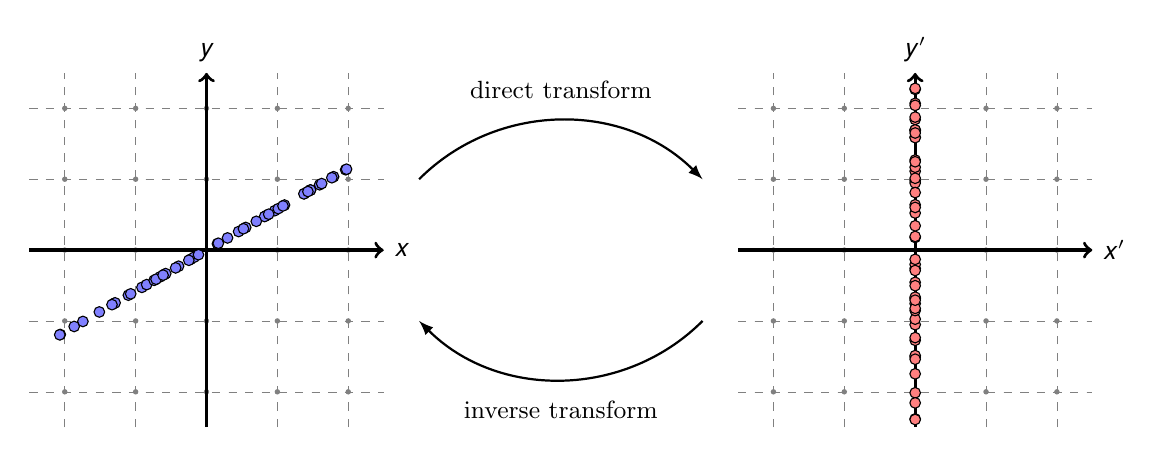
\begin{tikzpicture}[scale=0.9]
\tikzstyle{every node}=[font=\small]

	\draw[style=help lines, dashed, very thin, rotate=0] (0.5,0.5) grid (5.5,5.5);
	\draw[style=help lines, dashed, very thin, rotate=0] (10.5,0.5) grid (15.5,5.5);

	\foreach \x in {1,2,...,5} {
		\foreach \y in {1,2,...,5} {
			\filldraw [black!50, opacity = 1] (\x,\y) circle (0.03);
		}
	}

	\foreach \x in {11,12,...,15} {
		\foreach \y in {1,2,...,5} {
			\filldraw [black!50, opacity = 1] (\x,\y) circle (0.03);
		}
	}

	\def\seed{88}
	\pgfmathsetmacro{\xvar}{2.4}
	\pgfmathsetmacro{\yvar}{0.0}

	\def\angle{30}
	\pgfmathsetseed{\seed}
	\pgfmathsetmacro{\xoff}{3}
	\pgfmathsetmacro{\yoff}{3}
	\draw[style=help lines, dashed, very thin, rotate=0]
		(\xoff-2.5,\yoff-2.5) grid (\xoff+2.5,\yoff+2.5);
	\draw[->,very thick] (\xoff-2.5,\yoff)--(\xoff+2.5,\yoff) node[right]{$x$};
	\draw[->,very thick] (\xoff,\yoff-2.5)--(\xoff,\yoff+2.5) node[above]{$y$};
	\pgfmathsetmacro{\radius}{0.075}
	\foreach \i in {1,2,...,50} {
		\pgfmathsetmacro{\x}{(rand) * \xvar}
		\pgfmathsetmacro{\y}{(rand) * \yvar}
		\pgfmathsetmacro{\xrot}{\x*cos(\angle) - \y*sin(\angle) + \xoff}
		\pgfmathsetmacro{\yrot}{\x*sin(\angle) + \y*cos(\angle) + \yoff}
		\filldraw [black, fill=blue!50] (\xrot,\yrot) circle (\radius);
	}

	\def\angle{90}
	\pgfmathsetseed{\seed}
	\pgfmathsetmacro{\xoff}{13}
	\pgfmathsetmacro{\yoff}{3}
	\draw[style=help lines, dashed, very thin, rotate=0]
		(\xoff-2.5,\yoff-2.5) grid (\xoff+2.5,\yoff+2.5);
	\draw[->,very thick] (\xoff-2.5,\yoff)--(\xoff+2.5,\yoff) node[right]{$x'$};
	\draw[->,very thick] (\xoff,\yoff-2.5)--(\xoff,\yoff+2.5) node[above]{$y'$};
	\foreach \i in {1,2,...,50} {
		\pgfmathsetmacro{\x}{(rand) * \xvar}
		\pgfmathsetmacro{\y}{(rand) * \yvar}
		\pgfmathsetmacro{\xrot}{\x*cos(\angle) - \y*sin(\angle) + \xoff}
		\pgfmathsetmacro{\yrot}{\x*sin(\angle) + \y*cos(\angle) + \yoff}
		\filldraw [black, fill=red!50] (\xrot,\yrot) circle (\radius);
	}

	\draw [thick,-latex] (6,4) to [in=135,out=45] ++ (4,0);
	\draw [thick,latex-] (6,2) to [in=-135,out=-45] ++ (4,0);
	\node [above] at (8,5) {direct transform};
	\node [below] at (8,1) {inverse transform};
\end{tikzpicture}
% \end{document}

	\end{minipage}
\end{frame}
\begin{frame}{Separability and non-separability}
	\begin{block}{Pros \& Cons}
		\begin{minipage}{0.48\textwidth}
			\begin{block}{Non-separable}
				\begin{itemize}
					\item Able to exploit any linear correlation within a
						block
					\item They require $\approx N^4$ operations
				\end{itemize}
			\end{block}
		\end{minipage}
		\hfill
		\begin{minipage}{0.48\textwidth}
			\begin{block}{Separable}
				\begin{itemize}
					\item Able to decorrelate pixels sharing
						rows or columns
					\item They require $\approx 2 N^3$ operations
				\end{itemize}
			\end{block}
		\end{minipage}
	\end{block}
	\only<1>{\input{./figures/block_linearisation_1.tex}}
	\only<2>{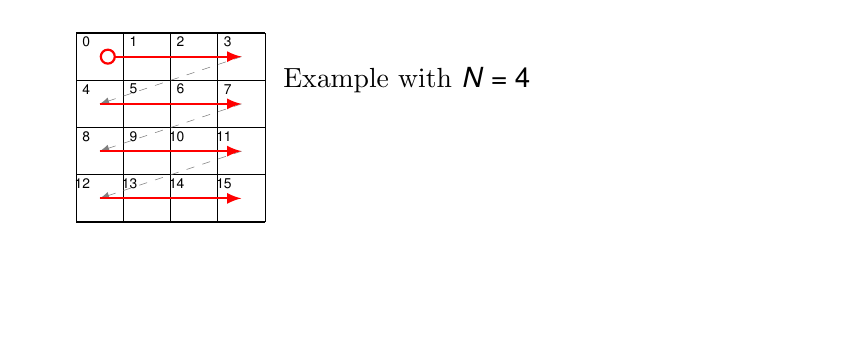
\begin{tikzpicture}[scale=0.6]

\def \xmax{4}
\def \ymax{4}
\draw[ystep=1, xstep=1]
	(0,0) grid (\xmax,\ymax);

\foreach \y in {0.5,1.5,...,\ymax}
{%
    \foreach \x in {0.5,1.5,...,\xmax}
    {%
      % floor the positions, as they are .5 and reverse vertical order
      \pgfmathtruncatemacro{\posX}{\x}
      \pgfmathtruncatemacro{\posY}{\ymax-\y}
      % calculate the index for each position
      \pgfmathtruncatemacro{\index}{\posX + \xmax * \posY}
      \node[above left] at (\x,\y){\tiny$\quad\quad\index$};
    }
}

\node at (7,3) {Example with $N=4$};

\def\startx{0.5}
\def\starty{3.5}

% help lines
\draw[latex-,style=help lines, dashed] (\startx + 0,\starty - 1) --++ (3,1);
\draw[latex-,style=help lines, dashed] (\startx + 0,\starty - 2) --++ (3,1);
\draw[latex-,style=help lines, dashed] (\startx + 0,\starty - 3) --++ (3,1);

% scanning
\draw[o-latex,style=help lines, red, thick] (\startx,\starty - 0) --++ ( 3,0);
\draw[-latex,style=help lines, red, thick] (\startx,\starty - 1) --++ ( 3,0);
\draw[-latex,style=help lines, red, thick] (\startx,\starty - 2) --++ ( 3,0);
\draw[-latex,style=help lines, red, thick] (\startx,\starty - 3) --++ ( 3,0);

\def \xmax{16}
\def \ymax{1}
\def\startx{0}
\def\starty{-2}

\draw[ystep=1, xstep=1,black!0]
	(\startx,\starty) grid (\startx+\xmax,\starty+\ymax);
% \foreach \x in {0,1,...,15}
% {%
%     \node[above left] at (\x+\startx+0.5,\starty+0.5) {\tiny$\quad\quad\x$};
% }

\draw[o-latex,style=help lines,red!0,thick] (\startx+0.5,\starty+0.5) --++ (\xmax-1,0);

\end{tikzpicture}
}
	\only<3>{\input{./figures/block_linearisation_3.tex}}
\end{frame}

\begin{frame}{What kind of data is processed by transforms?}
	\framesubtitle{Particular case of HEVC}
	\begin{minipage}{0.38\textwidth}
		\begin{block}{Residual blocks}
			\begin{itemize}
				\item Difference between:
					\begin{itemize}
						\item original block
						\item predicted block
					\end{itemize}
				\item Examples:\\[0.5em]
					\includegraphics[width=0.25\textwidth]{./figures/res_ipm10.png}
					\hfill
					\includegraphics[width=0.25\textwidth]{./figures/res_ipm18.png}
					\hfill
					\includegraphics[width=0.25\textwidth]{./figures/res_ipm26.png}
				\item The same transform is used for all of them
			\end{itemize}
		\end{block}
	\end{minipage}
	\hfill
	\begin{minipage}{0.58\textwidth}
		\begin{block}{They are generated as different combinations of}
			\begin{itemize}
				\item transform units (TUs): 32, 16, 8, 4
				\item predictions
					\begin{itemize}
						\item spatial or intra: 0,1,\ldots,34
						\item temporal or inter
					\end{itemize}
			\end{itemize}
		\end{block}
		\begin{block}{The choice is made by the encoder}
			\begin{itemize}
				\item it selects the best combination in terms of:
					\begin{itemize}
						\item distortion
						\item rate
					\end{itemize}
			\end{itemize}
		\end{block}
	\end{minipage}
\end{frame}

\begin{frame}{The intra prediction scheme}
	\framesubtitle{Intra Prediction Modes (IPMs)}
	\begin{minipage}{0.48\textwidth}
		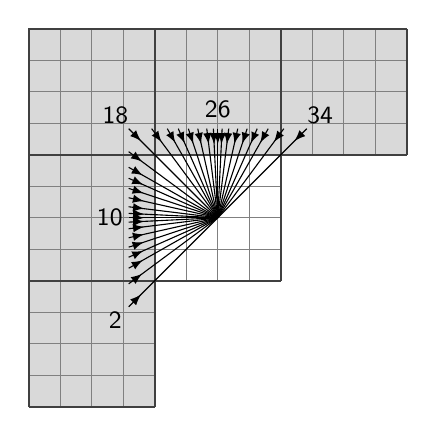
\begin{tikzpicture}[scale=1.60]

	\tikzset{middlearrow/.style={
		decoration={markings,
			mark= at position 0.95 with {\arrow{#1}} ,
		},
		postaction={decorate}
	}
}

	\def\startangle{45}
	\def\radius{0.707106781}

	\filldraw[fill=black!15, draw=black!75] (-6,-2) rectangle (-5,-1);
	\filldraw[fill=black!15, draw=black!75] (-6,-1) rectangle (-5,0);
	\filldraw[fill=black!15, draw=black!75] (-5,-1) rectangle (-4,0);
	\filldraw[fill=black!15, draw=black!75] (-6,-2) rectangle (-5,-3);
	\filldraw[fill=black!15, draw=black!75] (-4,0) rectangle (-3,-1);

	\draw[step=0.25,help lines] (-6,-2) grid (-4,0);
	\draw[step=0.25,help lines] (-6,-2) grid (-5,-3);
	\draw[step=0.25,help lines] (-4,0) grid (-3,-1);
	\draw[step=1,black!75,thick] (-6,-2) grid (-4,0);
	\draw[step=1,black!75,thick] (-6,-2) grid (-5,-3);
	\draw[step=1,black!75,thick] (-4,0) grid (-3,-1);

	% \foreach \direction in {2,3,...,34}
	\newcounter{dir}
	\setcounter{dir}{2}
    \foreach \position in {-32, -26, -21, -17, -13, -9, -5, -2, 0, 2, 5, 9,
	13, 17, 21, 26, 32, -26, -21, -17, -13, -9, -5, -2, 0, 2, 5, 9, 13, 17,
	21, 26, 32}
	{%
		% set the angle of current prediction direction 
		\pgfmathsetmacro{\angle}{\startangle - (\thedir - 2) * 180 / 32 + 180}
        \ifthenelse{\thedir < 19}
		{\pgfmathsetmacro{\angle}{-\position / 32 * 45 + 180}}
		{\pgfmathsetmacro{\angle}{-90 - \position / 32 * 45 + 180}}
		\ifthenelse{\thedir < 18}{\def\oper{cos}}{\def\oper{sin}}
		\pgfmathsetmacro{\radnew}{abs(\radius / \oper(\angle))}
		\ifthenelse{\thedir = 2 \OR \thedir = 10 \OR \thedir = 18 \OR \thedir = 26 \OR \thedir = 34}
		{\draw[opacity=0] (-4.5,-1.5) --++ (\angle:\radnew + 0.15) node
		[opacity=1] {\small \textsf{\thedir}};}{}

		\draw[middlearrow={latex reversed}] (-4.5,-1.5) --++ (\angle:\radnew);

		% update direction for next iteration
		\stepcounter{dir}
	}
\end{tikzpicture}

	\end{minipage}
	\begin{minipage}{0.48\textwidth}
		\includegraphics[width=0.25\textwidth]{./figures/residuals_4_10.png}
		\hfill \small Average residual for IPM 10

		\vspace{1em}

		\includegraphics[width=0.25\textwidth]{./figures/residuals_4_18.png}
		\hfill \small Average residual for IPM 18

		\vspace{1em}

		\includegraphics[width=0.25\textwidth]{./figures/residuals_4_26.png}
		\hfill \small Average residual for IPM 26
	\end{minipage}
\end{frame}

\subsection{Transform design}

\begin{frame}{How are transforms conceived?}
	\begin{block}{The trade-off}
		$J(\lambda) = \text{Distortion} + \lambda \; \text{Rate}$
	\end{block}
	\begin{block}{State of the art}
		\begin{itemize}
			\item KLT $\to$ Optimal transform assuming
				\begin{itemize}
					\item large amount of bits $\to$ High-resolution
						quantisation hypothesis
				\end{itemize}
			\item Hypothesis for optimality is not valid in video
				coding
			\item RDOT $\to$ Alternative design approach$^{[1]}$
				\begin{itemize}
					\item focused on signal sparsity in the transform domain
				\end{itemize}
		\end{itemize}
	\end{block}
	\begin{block}{References}
		\scriptsize
		% $[1]$ A. Arrufat --- Non-separable mode-dependent transforms for intra
		% coding in HEVC \\
		$[1]$ O.G. Sezer --- Sparse orthonormal transforms for image
		compression, 2008\\
	\end{block}
\end{frame}

\begin{frame}{The rate-distortion optimised transform}
	\begin{block}{RDOT design features}
		\begin{itemize}
			\item Minimise the distortion and the number of significant coefficients
			\item Use a simple model for the bit-rate
				\begin{itemize}
					\item $\ell_0$ norm: number of non-zero coefficients
				\end{itemize}
			\item Sparsity suits video coding syntax elements
		\end{itemize}
	\end{block}
	\begin{block}{The RDOT equation}
		\vspace{-4em}
		$$J(\lambda)=\sum_{\forall i}
		\underbrace{{\Vert\x_i-\A^T\cdot
		\c_i\Vert}^2}_{\text{Distortion}}
		+\lambda
		\underbrace{{\Vert\c_i\Vert}_0}_{\text{rate}}
		\qquad\text{with}
		\begin{cases}
			\x_i & \text{\small residuals}\\
			\A   & \text{\small transform}\\
			\c_i & \text{\small transf.\ \& quant.\ coeff.}\\
			\lambda & \text{\small Lagrange multiplier \tiny (PDF independent)}
		\end{cases}$$
	\end{block}
	\vspace{-2em}
	\begin{itemize}
		\item iterative algorithm
	\end{itemize}
	\begin{block}{Objective}
		\vspace{-0.5em}
		\begin{itemize}
			\item For a given set of residuals $\x_i$'s
			\item Find the transform $\A$ that minimises $J(\lambda)$
		\end{itemize}
	\end{block}
\end{frame}

\begin{frame}{RDOT metric for different transforms on $4\times4$ residuals}
	\vfill
	\only<1>{\input{./figures/rdot_learning_4_1_plot.tex}}
	\only<2>{\input{./figures/rdot_learning_4_2_plot.tex}}
	\only<3>{\input{./figures/rdot_learning_4_3_plot.tex}}
	\only<4>{\begin{tikzpicture}
	\pgfplotsset{/tikz/font={\scriptsize}}
	\begin{axis}[
			xlabel={iteration},
			ylabel={RDOT metric},
			grid=both,
			scale only axis,
			width=0.8\textwidth,
			height=0.7\textheight,
			scaled y ticks = false,
			x tick label style={
				/pgf/number format/.cd,
				set thousands separator={\thinspace},
				set decimal separator={.},
				fixed,
				fixed zerofill,
				precision=0,
				/tikz/.cd
			},
			y tick label style={
				/pgf/number format/.cd,
				set decimal separator={.},
				fixed,
				fixed zerofill,
				precision=1,
				/tikz/.cd
			},
			% xtick={0.20,0.22,...,0.50},
			ytick={0,0.5,...,100},
			xmin=0, xmax=1000,
			ymin=33, ymax=36.5,
			legend style={nodes=right},
			legend pos= north east,
			unbounded coords=jump,
		]

		\pgfplotstableread{figures/rdot_learning_4.dat}\table
		\addplot[black, dotted, thick]
		table[x=iter,y=dct,col sep=tab] from \table;
		\addlegendentry{DCT-II}

		\pgfplotstableread{figures/rdot_learning_4.dat}\table
		\addplot[black, dashed, thick]
		table[x=iter,y=dst,col sep=tab] from \table;
		\addlegendentry{DST-VII}

		\pgfplotstableread{figures/rdot_learning_4.dat}\table
		\addplot[blue, dashed, thick, smooth]
		table[x=iter,y=klt_sep,col sep=tab] from \table;
		\addlegendentry{KLT}

		\pgfplotstableread{figures/rdot_learning_4.dat}\table
		\addplot[blue, thick]
		table[x=iter,y=klt_nsep,col sep=tab] from \table;
		\addlegendentry{NS-KLT}

		% \pgfplotstableread{figures/rdot_learning_4.dat}\table
		% \addplot[red, dashed, thick]
		% table[x=iter,y=rdot_sep,col sep=tab] from \table;
		% \addlegendentry{RDOT}

		% \pgfplotstableread{figures/rdot_learning_4.dat}\table
		% \addplot[red, thick, smooth]
		% table[x=iter,y=rdot_nsep,col sep=tab] from \table;
		% \addlegendentry{NS-RDOT}

	\end{axis}

\end{tikzpicture}
}
	\only<5>{\input{./figures/rdot_learning_4_5_plot.tex}}
	\only<6>{\input{./figures/rdot_learning_4_6_plot.tex}}
\end{frame}

\begin{frame}{Experiment: Using the transforms in HEVC}
	\only<1>{
	\framesubtitle{Mode-dependent directional transforms (MDDT) for $4\times4$
	and $8\times8$ TUs}
	\begin{block}{Learning phase}
		\vspace{-0.5em}
		\begin{itemize}
			\item Learn an adapted transform to each of the 35 IPMs (MDDT)
			\item Replace the default HEVC transforms (no additional
				signalling) with:
				\begin{itemize}
					\item KLT
					\item RDOT
				\end{itemize}
		\end{itemize}
	\end{block}
	\vspace{-0.5em}
	\begin{block}{Decoding scheme}
		\vspace{0.5em}
		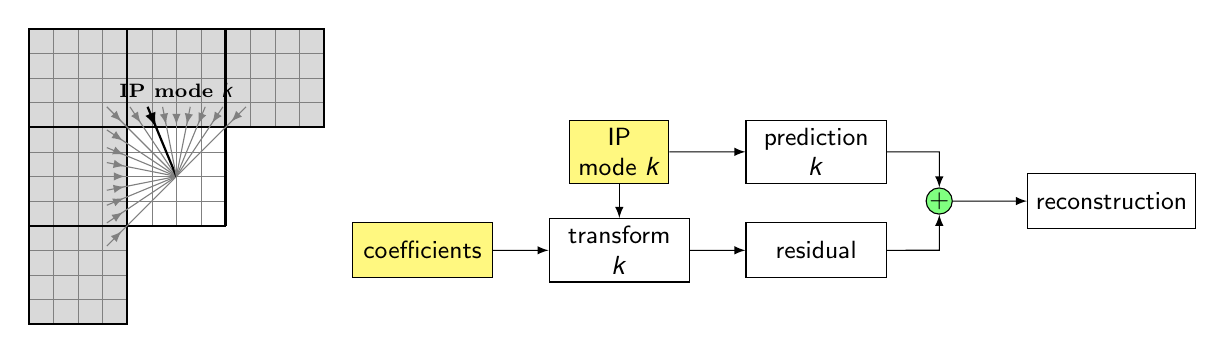
\begin{tikzpicture}[scale=1.25]
\tikzstyle{every node}=[font=\small]
	\tikzset{middlearrow/.style={
		decoration={markings,
			mark= at position 0.9 with {\arrow{#1}} ,
		},
		postaction={decorate}
	}
}

	\def\startx{0}
	\def\starty{0}
	\def\radius{3.0}
	\def\startangle{45}
	\def\colour{black}
	\def\thickness{help lines}
	\def\hdist{2}
	\def\startangle{45}
	\def\radius{0.707}
	\def\thickness{black!50}
	\def\selmode{ }
	\pgfmathsetmacro{\nodebasesize}{1} % A node with a value of one will have this diameter
	\pgfmathsetmacro{\nodeinnersep}{0.1}
	\tikzstyle{bloq} = [rectangle, draw, text badly centered, minimum height=2em, inner sep=1mm]
	\newcommand{\bloq}[4]{% position, name options,
		label \node[bloq,#3](#2) at (#1) {\textsf{#4}};
	}
	\newcommand{\propnode}[5]{% position, name, options, value, label
		\pgfmathsetmacro{\minimalwidth}{sqrt(#4*\nodebasesize)}
		\node[#3,minimum width=\minimalwidth*1cm,inner sep=\nodeinnersep*0cm,circle,draw] 
		(#2) at (#1) {#5};
	}

	\tikzstyle{frame} =
	[rectangle, fill=white, draw, text centered, minimum width=4em, minimum height=2em]

	\filldraw[fill=black!15, draw=black] (-6,-2) rectangle (-5,-1);
	\filldraw[fill=black!15, draw=black] (-6,-1) rectangle (-5,0);
	\filldraw[fill=black!15, draw=black] (-5,-1) rectangle (-4,0);
	\filldraw[fill=black!15, draw=black] (-6,-2) rectangle (-5,-3);
	\filldraw[fill=black!15, draw=black] (-4,0) rectangle (-3,-1);

	\draw[step=0.25,help lines] (-6,-2) grid (-4,0);
	\draw[step=0.25,help lines] (-6,-2) grid (-5,-3);
	\draw[step=0.25,help lines] (-4,0) grid (-3,-1);
	\draw[step=1,black,thick] (-6,-2) grid (-4,0);
	\draw[step=1,black,thick] (-6,-2) grid (-5,-3);
	\draw[step=1,black,thick] (-4,0) grid (-3,-1);

	\foreach \direction in {2,4,...,34}
	{%
		% set the angle of current prediction direction 
		\pgfmathsetmacro{\angle}{\startangle - (\direction - 2) * 180 / 32 + 180}
		\ifthenelse{\direction < 18}{\def\oper{cos}}{\def\oper{sin}}
		\pgfmathsetmacro{\radnew}{abs(\radius / \oper(\angle))}
		% draw the prediction direction lines with the appropriate colour
		\ifthenelse{\direction = 22}{\def\thickness{thick}\def\selmode{$k$}};
		\draw[\colour, \thickness, middlearrow={latex reversed}] (-4.5,-1.5) --++ (\angle:\radnew);
	}

	\draw(-4.5,-0.80) node[above] {\scriptsize \bf IP mode $k$};

	%\draw[-latex] (-2,-1.5) to [in=180,out= 00] ++ (1.30,0.25);
	%\draw[-latex] (-2,-1.5) to [in=180,out= 00] ++ (1.30,-0.75);

	%\draw (-4.5,-3.05) node[below] {\scriptsize Block to predict and decode};


	\draw[dotted](\startx,\starty -0.5) ++ (0,-2);

	\bloq{\startx,\starty-1.25}{ipk}{text width=3em,fill=yellow!50}{IP mode $k$}
	\bloq{\startx-\hdist,\starty-2.25}{coefk}{text width=4.5em,fill=yellow!50}{coefficients}

	\bloq{\startx+\hdist,\starty-1.25}{predk}{text width=4.5em}{prediction $k$}
	\bloq{\startx,\starty-2.25}{trk}{text width=4.5em}{transform $k$}

	\bloq{\startx+\hdist,\starty-2.25}{res}{text width=4.5em}{residual}

	\bloq{\startx+2.5*\hdist,\starty-1.75}{rec}{text width=5.5em}{reconstruction}

	\draw[-latex] (ipk) -- (predk);
	
	\draw[-latex] (ipk) -- (trk);

	\draw[-latex] (coefk) -- (trk);

	\draw[-latex] (trk) -- (res);

	\propnode{3.25,-1.75}{add1}{fill=green!50}{0}{\small+}

	\draw[-latex] (predk) --++ (1,0) -| (add1);
	\draw[-latex] (res) --++ (1,0) -| (add1);
	\draw[-latex] (add1) -- (rec);

\end{tikzpicture}

% vim:set filetype=tex:

	\end{block}}
	% \only<2>{
	% \framesubtitle{Common Test Conditions used at JCT-VC}
	% \begin{block}{Guidelines used to compare video encoding performances}
	% 	\vspace{-0.5em}
	% 	\begin{itemize}
	% 		\item Encode sequences at 4 different qualities (QP 22, 27, 32,
	% 			37)
	% 		\item Measure the bit-rate savings (BD-rate) in \%. Example:
	% 			-16.39\%
	% 	\end{itemize}
	% 	\vspace{-0.5em}
	% 	\begin{center}
	% 		\input{./figures/bd_rate_plot.tex}
	% 	\end{center}
	% \end{block}
	% }
\end{frame}

\begin{frame}{MDDT performances on the HEVC test set}
	\framesubtitle{Y BD-rate (\%) on AI for $4\times4$ and $8\times8$ blocks}
	
\begin{tikzpicture}
	\pgfplotsset{/tikz/font={\small}}
	\begin{axis}[
		grid=both,
		width=1.0\textwidth,
		height=0.3\textheight,
		x tick label style={
		/pgf/number format/1000 sep=},
		ytick={0,-2,...,-12},
		y tick label style={
			/pgf/number format/.cd,
			fixed,
			fixed zerofill,
			precision=1,
		},
		y dir=reverse,
		ymax=1, ymin=-12,
		ylabel={Y BD-rate (\%)},
		% enlargelimits=0.15,
		enlarge y limits=false,
		enlarge x limits=0.04,
		legend style={at={(0.5,-0.45)},
		anchor=north,legend columns=-1},
		ybar,
		bar width=1pt,
		xtick=data,
		xtick align=inside,
		% nodes near coords,
		% xlabel={Sequences},
		% xlabel near ticks,
		symbolic x coords={
			NebutaFestival,
			PeopleOnStreet,
			SteamLocTrain,
			Traffic,
			BasketballDrive,
			BQTerrace,
			Cactus,
			Kimono1,
			ParkScene,
			BasketballDrill,
			BQMall,
			PartyScene,
			RaceHorses\_480p,
			BasketballPass,
			BlowingBubbles,
			BQSquare,
			RaceHorses\_240p,
			FourPeople,
			Johnny,
			KristenAndSara,
			BasketDrillText,
			ChinaSpeed,
			SlideEditing,
			SlideShow,
			Overall,
		},
		x tick label style={rotate=-60,anchor=west},
		]

		\addlegendentry{Sep KLT AI}
		\addplot coordinates {
		(NebutaFestival,   -0.55)
		(PeopleOnStreet,   -1.17)
		(SteamLocTrain,    -0.50)
		(Traffic,          -1.33)
		(BasketballDrive,   0.12)
		(BQTerrace,         0.27)
		(Cactus,           -0.92)
		(Kimono1,          -0.38)
		(ParkScene,        -1.19)
		(BasketballDrill,  -1.20)
		(BQMall,            0.03)
		(PartyScene,       -0.04)
		(RaceHorses\_480p, -0.84)
		(BasketballPass,   -0.11)
		(BlowingBubbles,   -0.05)
		(BQSquare,          0.09)
		(RaceHorses\_240p, -1.00)
		(FourPeople,       -1.19)
		(Johnny,           -0.33)
		(KristenAndSara,   -0.18)
		(BasketDrillText,  -0.84)
		(ChinaSpeed,        0.44)
		(SlideEditing,      0.68)
		(SlideShow,         0.73)
		(Overall,          -0.39)
		};

		\addlegendentry{Sep RDOT AI}
		\addplot coordinates {
		(NebutaFestival,   -0.37)
		(PeopleOnStreet,   -1.31)
		(SteamLocTrain,    -0.41)
		(Traffic,          -1.49)
		(BasketballDrive,  -0.59)
		(BQTerrace,        -0.85)
		(Cactus,           -1.47)
		(Kimono1,          -0.47)
		(ParkScene,        -1.28)
		(BasketballDrill,  -1.77)
		(BQMall,           -1.14)
		(PartyScene,       -1.15)
		(RaceHorses\_480p, -1.26)
		(BasketballPass,   -0.94)
		(BlowingBubbles,   -0.97)
		(BQSquare,         -1.00)
		(RaceHorses\_240p, -1.34)
		(FourPeople,       -1.51)
		(Johnny,           -0.75)
		(KristenAndSara,   -0.59)
		(BasketDrillText,  -1.80)
		(ChinaSpeed,       -0.81)
		(SlideEditing,     -0.57)
		(SlideShow,        -0.55)
		(Overall,          -1.02)
		};

		\addlegendentry{N-sep KLT AI}
		\addplot coordinates {
		(NebutaFestival,  -0.72)
		(PeopleOnStreet,  -2.53)
		(SteamLocTrain,   -0.60)
		(Traffic,         -2.66)
		(BasketballDrive, -1.12)
		(BQTerrace,       -2.19)
		(Cactus,          -2.28)
		(Kimono1,         -0.95)
		(ParkScene,       -1.69)
		(BasketballDrill, -7.92)
		(BQMall,          -0.83)
		(PartyScene,      -1.00)
		(RaceHorses\_480p,-2.60)
		(BasketballPass,  -1.47)
		(BlowingBubbles,  -1.80)
		(BQSquare,        -0.91)
		(RaceHorses\_240p,-3.36)
		(FourPeople,      -2.41)
		(Johnny,          -1.52)
		(KristenAndSara,  -1.56)
		(BasketDrillText, -6.14)
		(ChinaSpeed,      -0.02)
		(SlideEditing,     0.98)
		(SlideShow,        0.37)
		(Overall,         -1.87)
		};

		\addlegendentry{N-sep RDOT AI}
		\addplot coordinates {
		(NebutaFestival,   -0.44)
		(PeopleOnStreet,   -2.50)
		(SteamLocTrain,    -0.55)
		(Traffic,          -2.90)
		(BasketballDrive,  -2.82)
		(BQTerrace,        -4.62)
		(Cactus,           -3.41)
		(Kimono1,          -1.11)
		(ParkScene,        -1.92)
		(BasketballDrill, -11.88)
		(BQMall,           -2.58)
		(PartyScene,       -2.56)
		(RaceHorses\_480p, -3.57)
		(BasketballPass,   -3.12)
		(BlowingBubbles,   -3.49)
		(BQSquare,         -2.69)
		(RaceHorses\_240p, -4.34)
		(FourPeople,       -3.20)
		(Johnny,           -2.82)
		(KristenAndSara,   -2.99)
		(BasketDrillText,  -9.96)
		(ChinaSpeed,       -1.81)
		(SlideEditing,     -0.46)
		(SlideShow,        -1.81)
		(Overall,          -3.23)
		};

	\end{axis}
\end{tikzpicture}

\end{frame}

\begin{frame}{Conclusions}
	\begin{block}{Performance over HEVC}
		\scriptsize
		\centering
		\begin{tabular}{c|rr|rr}
			\multicolumn{1}{c}{}
			& \multicolumn{2}{c|}{KLT}
			& \multicolumn{2}{c}{RDOT} \\
			\multicolumn{1}{c}{}
			& \multicolumn{1}{c}{sep} & \multicolumn{1}{c|}{non-sep}
			& \multicolumn{1}{c}{sep} & \multicolumn{1}{c}{non-sep} \\
			\hline\hline
			Y BD-rate & -0.39\% & -1.87\% & -1.02\% & -3.23\% \\
			Encoding  & 108\% & 112\% & 108\% & 112\% \\
			Decoding  & 105\% & 120\% & 105\% & 120\% \\
			ROM &
			\SI{8.20}{\kilo B} & \SI{148.75}{\kilo B} &
			\SI{8.20}{\kilo B} & \SI{148.75}{\kilo B}\\
		\end{tabular}
	\end{block}

	\begin{block}{Transform design}
		\begin{itemize}
			\item RDOT design provides significant better results than the KLT
				design
			\item Separability plays an important role on the performance
				\begin{itemize}
					\item complexity (encoding/decoding)
					\item storage requirements
					\item bit-rate savings
				\end{itemize}
		\end{itemize}
	\end{block}
	\begin{block}{Next steps}
		\begin{itemize}
			\item Find out the limits of this technique
		\end{itemize}
	\end{block}
\end{frame}

\section[MDTC]{Mode-dependent transform competition}

\begin{frame}{Mode-dependent transform competition (MDTC)}
	\begin{block}{Motivations}
		\begin{itemize}
			\item Residual variability even inside the same IPM
			\item Significantly better results using RDOTs in MDDT than KLTs
		\end{itemize}
	\end{block}
	\begin{block}{Multiple transform design for HEVC}
		\begin{itemize}
			\item Conservative approach $\to$ $1+2^N$ transforms
				\begin{itemize}
					\item default transform (DCT/DST) + additional RDOTs
					\item signalling $\to$ flag plus fixed length codeword
				\end{itemize}
			\item Learning algorithm $\to$ based on the RDOT metric
		\end{itemize}
	\end{block}
\end{frame}

\subsection{Multiple transform design}
\begin{frame}{\currentname}
	\framesubtitle{Classic clustering method: classify/update}
	\begin{minipage}{0.49\textwidth}
		\small
		\begin{block}{Using the RDOT metric}
			\begin{itemize}
				\item $J(\lambda)=\displaystyle\sum_{\forall i}
					{\Vert\x_i-\A^T\cdot \c_i\Vert}^2
					+\lambda {\Vert\c_i\Vert}_0$
				\item It is used to evaluate a transform
					\begin{itemize}
						\scriptsize
						\item compute the optimal transform for a set of
							residuals
						\item assign each residual to the transform that
							minimises $J(\lambda)$
					\end{itemize}
				\item It allows creating an iterative clustering algorithm
			\end{itemize}
		\end{block}
	\end{minipage}
	\hfill
	\begin{minipage}{0.49\textwidth}
		\includegraphics[width=\textwidth]{./figures/clustering.pdf}
	\end{minipage}
\end{frame}

\begin{frame}{Learning results}
	\only<1>{
	\framesubtitle{Averaged RDOT metric for $4\times4$ blocks across all IPMs}
	\vspace{1em}
	\begin{tikzpicture}
	\pgfplotsset{/tikz/font={\footnotesize}}
	\begin{axis}[
			% title=Bitrate savings: $-8.94\%$. SNR improvement: $0.46$ dB,
			% xlabel={Number of $4\times4$ transforms},
			ylabel={RDOT metric},
			grid=both,
			scale only axis,
			width=0.8\textwidth,
			height=0.2\textheight,
			xtick={0,1,2,4,8,16},
			x tick label style={
				rotate=-45, anchor=west,
				/pgf/number format/.cd,
				fixed,
				fixed zerofill,
				precision=0,
			},
			xlabel near ticks,
			scaled x ticks=false,
			ytick={0,1,...,99},
			y tick label style={
				/pgf/number format/.cd,
				fixed,
				fixed zerofill,
				precision=1,
				/tikz/.cd
			},
			xmin=0, xmax=16,
			ymin=25, ymax=35,
			legend style={nodes=right},
			legend pos= north east,
            xticklabels={DST, DST + 1 RDOT, DST + 2 RDOT, DST + 4 RDOT, DST + 8 RDOT, DST+ 16 RDOT},
		]

		% 1	34.32
		\addplot [mark=*,mark size=1pt, red, thick, dashed] table {
		0	34.95
		1	32.11
		2	30.88
		4	29.61
		8	28.34
		16	27.16
		};
		\addlegendentry{Separable}

		% 1	32.21
		\addplot [mark=*,mark size=1pt, red, thick] table {
		0	34.95
		1	31.19
		2	29.81
		4	28.40
		8	26.84
		16	25.68
		};
		\addlegendentry{Non-separable}

		\end{axis}
	\end{tikzpicture}

	}
	% \only<2>{
	% \framesubtitle{Averaged RDOT metric for $8\times8$ blocks}
	% \vspace{1em}
	% \begin{tikzpicture}
	\pgfplotsset{/tikz/font={\tiny}}
	\begin{axis}[
			% title=Bitrate savings: $-8.94\%$. SNR improvement: $0.46$ dB,
			% xlabel={Number of $8\times8$ transforms},
			grid=both,
			scale only axis,
			width=0.9\textwidth,
			height=0.6\textheight,
			xtick={0,1,2,4,8,16,32},
			x tick label style={
				rotate=-60, anchor=west,
				/pgf/number format/.cd,
				fixed,
				fixed zerofill,
				precision=0,
			},
			xlabel near ticks,
			scaled x ticks=false,
			ytick={0,1,...,99},
			y tick label style={
				/pgf/number format/.cd,
				fixed,
				fixed zerofill,
				precision=0,
				/tikz/.cd
			},
			xmin=0, xmax=32,
			ymin=19, ymax=28,
			legend style={nodes=right},
			legend pos= north east,
            xticklabels={DCT, DCT + 1 RDOT, DCT + 2RDOT, DCT + 4 RDOT, DCT + 8 RDOT,
			DCT + 16 RDOT, DCT + 32 RDOT},
		]

		% 1	25.97
		\addplot [mark=*,mark size=1pt, red, thick, dashed] table {
		0	27.04
		1	25.00
		2	24.28
		4	23.62
		8	23.03
		16	22.37
		32	21.78
		};
		\addlegendentry{separable}

		% 1	24.38
		\addplot [mark=*,mark size=1pt, red, thick] table {
		0	27.04
		1	23.61
		2	22.81
		4	22.02
		8	21.26
		16	20.53
		32	19.82
		};
		\addlegendentry{non-separable}

		\end{axis}
	\end{tikzpicture}

	% }
\end{frame}

\subsection{Results in video coding on top of HEVC}

\begin{frame}{\currentname}
	\only<1>{
	\framesubtitle{Y BD-rate (\%) for $4\times4$ blocks}
	\vspace{1em}
	\begin{tikzpicture}
	\pgfplotsset{/tikz/font={\small}}
	\begin{axis}[
			% xlabel={Additional $8\times8$ transforms},
			ylabel={Y BD-rate (\%)},
			grid=both,
			scale only axis,
			width=0.9\textwidth,
			height=0.2\textheight,
			xtick={0, 1, 2, 4, 8, 16},
			x tick label style={
				rotate=-90, anchor=west,
				/pgf/number format/.cd,
				fixed,
				fixed zerofill,
				precision=0,
			},
			y tick label style={
				/pgf/number format/.cd,
				fixed,
				fixed zerofill,
				precision=1,
			},
			ytick={0,-0.5,...,-4},
			% yticklabels={0\%, -1\%, -2\%, -3\%, -4\%, -5\%, -6\%},
			xmin=0, xmax=16,
			ymin=-2.5, ymax=0,
			% legend entries={sep-$8\times8$,nsep-$8\times8$},
			legend style={nodes=right},
			legend pos= north east,
            xticklabels={DST, DST + 1 RDOT, DST + 2RDOT, DST + 4 RDOT, DST + 8 RDOT,
			DST + 16 RDOT},
		]

		% \pgfplotstableread{figures/prog_transf_8x8.dat}\table
		% \addplot[mark=*,mark size=1.1pt, red, thick, smooth, tension=0.3, dashed]
		% table[x=ntrans,y=sep,col sep=tab] from \table;

		\addplot [mark=*,mark size=1pt, red, thick, dashed] table {
		0	0
		1	-0.79
		2	-1.06
		4	-1.28
		8	-1.42
		16	-1.54
		};
		\addlegendentry{separable}

		\addplot [mark=*,mark size=1pt, red, thick] table {
		0	0
		1	-1.75
		2	-2.09
		4	-2.28
		8	-2.34
		16	-2.44
		};
		\addlegendentry{non-separable}
	\end{axis}
\end{tikzpicture}

	}
	% \only<2>{
	% \framesubtitle{Bit-rate savings for $8\times8$ blocks}
	% \vspace{1em}
	% \begin{tikzpicture}
	\pgfplotsset{/tikz/font={\footnotesize}}
	\begin{axis}[
			% xlabel={Additional $8\times8$ transforms},
			ylabel={Y BD-rate (\%)},
			grid=both,
			scale only axis,
			width=0.8\textwidth,
			height=0.225\textheight,
			xtick={0, 1, 2, 4, 8, 16, 32},
			x tick label style={
				rotate=-45, anchor=west,
				/pgf/number format/.cd,
				fixed,
				fixed zerofill,
				precision=0,
			},
			% xticklabels={0, 1, 2, 4, 8, 16, 32},
			ytick={0,-1,-2,-3,-4,-5,-6},
			% yticklabels={0\%, -1\%, -2\%, -3\%, -4\%, -5\%, -6\%},
			xmin=0, xmax=32,
			ymin=-6, ymax=0,
			% legend entries={sep-$8\times8$,nsep-$8\times8$},
			legend style={nodes=right},
			legend pos= north east,
            xticklabels={DCT, DCT + 1 RDOT, DCT + 2RDOT, DCT + 4 RDOT, DCT + 8 RDOT,
			DCT + 16 RDOT, DCT + 32 RDOT},
		]

		% \pgfplotstableread{figures/prog_transf_8x8.dat}\table
		% \addplot[mark=*,mark size=1.1pt, red, thick, smooth, tension=0.3, dashed]
		% table[x=ntrans,y=sep,col sep=tab] from \table;

		\addplot [mark=*,mark size=1pt, red, thick, dashed] table {
		0	0
		1	-0.9910
		2	-1.4612
		4	-1.8767
		8	-2.2685
		16	-2.6962
		32	-3.1103
		};
		\addlegendentry{Separable}

		\addplot [mark=*,mark size=1pt, red, thick] table {
		0	0
		1	-2.8143
		2	-3.6062
		4	-4.2264
		8	-4.8164
		16	-5.3988
		32	-5.9602
		};
		\addlegendentry{Non-separable}
	\end{axis}
\end{tikzpicture}

% vim:set filetype=tex:

	% }
\end{frame}

\begin{frame}{MDTC performances in detail}
	\only<1>{
	\begin{block}{Y BD-rate (\%) for High Performance System:
		$4\times4:1+16\,\,\&\,\,8\times8:1+32$}
		\begin{tikzpicture}
	\pgfplotsset{/tikz/font={\small}}
	\begin{axis}[
		grid=both,
		width=1.0\textwidth,
		height=0.3\textheight,
		x tick label style={
		/pgf/number format/1000 sep=},
		ytick={0,-2,...,-26},
		y tick label style={
			/pgf/number format/.cd,
			fixed,
			fixed zerofill,
			precision=1,
		},
		y dir=reverse,
		ymax=0.5, ymin=-26,
		ylabel={Y BD-rate (\%)},
		% enlargelimits=0.15,
		enlarge y limits=false,
		enlarge x limits=0.04,
		legend style={at={(0.5,-0.45)},
		anchor=north,legend columns=-1},
		ybar,
		bar width=1pt,
		xtick=data,
		xtick align=inside,
		% nodes near coords,
		% xlabel={Sequences},
		% xlabel near ticks,
		symbolic x coords={
			NebutaFestival,
			PeopleOnStreet,
			SteamLocTrain,
			Traffic,
			BasketballDrive,
			BQTerrace,
			Cactus,
			Kimono1,
			ParkScene,
			BasketballDrill,
			BQMall,
			PartyScene,
			RaceHorses\_480p,
			BasketballPass,
			BlowingBubbles,
			BQSquare,
			RaceHorses\_240p,
			FourPeople,
			Johnny,
			KristenAndSara,
			BasketDrillText,
			ChinaSpeed,
			SlideEditing,
			SlideShow,
			Overall,
		},
		x tick label style={rotate=-60,anchor=west},
		]

		\addlegendentry{Sep AI}
		\addplot coordinates {
		(NebutaFestival,   -1.06)
		(PeopleOnStreet,   -4.21)
		(SteamLocTrain,    -0.60)
		(Traffic,          -4.52)
		(BasketballDrive,  -3.22)
		(BQTerrace,        -4.70)
		(Cactus,           -5.22)
		(Kimono1,          -1.10)
		(ParkScene,        -4.61)
		(BasketballDrill,  -5.92)
		(BQMall,           -4.79)
		(PartyScene,       -4.88)
		(RaceHorses\_480p, -4.25)
		(BasketballPass,   -3.91)
		(BlowingBubbles,   -4.30)
		(BQSquare,         -4.58)
		(RaceHorses\_240p, -3.85)
		(FourPeople,       -4.56)
		(Johnny,           -3.34)
		(KristenAndSara,   -3.82)
		(BasketDrillText,  -6.24)
		(ChinaSpeed,       -4.25)
		(SlideEditing,     -4.80)
		(SlideShow,        -5.66)
		(Overall,          -4.10)
		};

		\addlegendentry{Sep RA}
		\addplot coordinates {
		(NebutaFestival,   -0.08)
		(PeopleOnStreet,   -1.49)
		(SteamLocTrain,     0.23)
		(Traffic,          -3.73)
		(BasketballDrive,  -0.72)
		(BQTerrace,        -2.65)
		(Cactus,           -3.08)
		(Kimono1,          -0.79)
		(ParkScene,        -3.22)
		(BasketballDrill,  -3.53)
		(BQMall,           -2.79)
		(PartyScene,       -3.21)
		(RaceHorses\_480p, -1.59)
		(BasketballPass,   -1.82)
		(BlowingBubbles,   -2.69)
		(BQSquare,         -2.74)
		(RaceHorses\_240p, -1.54)
		(FourPeople,       -5.18)
		(Johnny,           -4.16)
		(KristenAndSara,   -4.47)
		(BasketDrillText,  -3.71)
		(ChinaSpeed,       -2.71)
		(SlideEditing,     -5.05)
		(SlideShow,        -5.61)
		(Overall,          -2.76)
		};

























		\addlegendentry{N-sep AI}
		\addplot coordinates {
		(NebutaFestival,   -1.15)
		(PeopleOnStreet,   -5.65)
		(SteamLocTrain,    -0.68)
		(Traffic,          -6.06)
		(BasketballDrive,  -5.52)
		(BQTerrace,        -9.22)
		(Cactus,          -10.92)
		(Kimono1,          -1.80)
		(ParkScene,        -5.27)
		(BasketballDrill, -25.06)
		(BQMall,           -6.21)
		(PartyScene,       -6.19)
		(RaceHorses\_480p, -6.75)
		(BasketballPass,   -6.15)
		(BlowingBubbles,   -6.73)
		(BQSquare,         -6.12)
		(RaceHorses\_240p, -7.13)
		(FourPeople,       -6.33)
		(Johnny,           -5.21)
		(KristenAndSara,   -6.01)
		(BasketDrillText, -21.64)
		(ChinaSpeed,       -4.86)
		(SlideEditing,     -3.67)
		(SlideShow,        -6.03)
		(Overall,          -7.10)
		};

		\addlegendentry{N-sep RA}
		\addplot coordinates {
		(NebutaFestival,   -0.13)
		(PeopleOnStreet,   -2.27)
		(SteamLocTrain,     0.03)
		(Traffic,          -5.12)
		(BasketballDrive,  -2.36)
		(BQTerrace,        -4.93)
		(Cactus,           -7.68)
		(Kimono1,          -1.18)
		(ParkScene,        -3.69)
		(BasketballDrill, -14.80)
		(BQMall,           -3.64)
		(PartyScene,       -4.30)
		(RaceHorses\_480p, -3.24)
		(BasketballPass,   -3.14)
		(BlowingBubbles,   -3.95)
		(BQSquare,         -3.61)
		(RaceHorses\_240p, -3.20)
		(FourPeople,       -6.70)
		(Johnny,           -5.78)
		(KristenAndSara,   -6.17)
		(BasketDrillText, -13.15)
		(ChinaSpeed,       -3.03)
		(SlideEditing,     -4.06)
		(SlideShow,        -5.91)
		(Overall,          -4.67)
		};

	\end{axis}
\end{tikzpicture}

	\end{block}}
	\only<2>{\framesubtitle{Graphical improvement at QP 37 on BasketballDrill
	(3 Mbps)}}
	\only<2>{
	\begin{figure}[tb]
		\centering
		\subfloat[Original]
		{\includegraphics[width=0.30\linewidth]
		{./figures/bdrill_orig_crop.png}}
		\hfill
		\subfloat[HEVC]
		{\includegraphics[width=0.30\linewidth]
		{./figures/bdrill_hevc_qp37_crop.png}}
		\hfill
		\subfloat[MDTC]
		{\includegraphics[width=0.30\linewidth]
		{./figures/bdrill_mdtc_qp37_crop.png}}
		\caption{Comparison between HEVC and MDTC}
	\end{figure}}
\end{frame}

\begin{frame}{Conclusions}
	\centering
	\begin{block}{Performances}
		\scriptsize
		\centering
		\begin{tabular}{ccc}
			\multicolumn{1}{c}{} &
			\multicolumn{2}{c}{\multirow{2}{2.75cm}{\centering $4\times4$: 1+16 $\quad 8\times8$: 1+32}} \\
			\multicolumn{1}{c}{} & & \\
			\cline{2-3}
			\multicolumn{1}{c}{} & \multicolumn{1}{c|}{sep.} & non-sep. \\
			\hline
			\hline
			\multicolumn{1}{c|}{Y BD-rate} & \multicolumn{1}{c|}{-4.10\%}   & -7.10\% \\
			\multicolumn{1}{c|}{Enc. Time} & \multicolumn{1}{c|}{800\%  }   & 2000\% \\
			\multicolumn{1}{c|}{Dec. Time} & \multicolumn{1}{c|}{105\%  }   & 120\% \\
			\multicolumn{1}{c|}{ROM}       & \multicolumn{1}{c|}{236.25 kB} & 4.51 MB \\
		\end{tabular}
	\end{block}
	\begin{block}{Next steps}
		\begin{itemize}
			\item Important bit-rate savings thanks to transform competition
			\item Non-separable transforms are very complex
				\begin{itemize}
					\item encoding/decoding complexity
					\item storage requirements
				\end{itemize}
			\item Simplify MDTC systems to make them usable
		\end{itemize}
	\end{block}
\end{frame}

\section[MDTC simplifications]{Simplifications of the MDTC systems}

\AtBeginSubsection[]
{
    \frame<handout:0>
    {
        \frametitle{Outline}
        \tableofcontents
        [sectionstyle=show/shaded,subsectionstyle=show/shaded/hide,
		subsubsectionstyle=hide/hide/hide]
    }
}

% \subsection{Incomplete transforms}

% \begin{frame}{\currentname}
% 	\begin{block}{Motivations}
% 		\begin{itemize}
% 			\item Use of non-separable transforms at low complexity
% 			\item Focus on decoding complexity
% 		\end{itemize}
% 	\end{block}
% 	\begin{minipage}{0.45\textwidth}
% 		\centering
% 		\only<1>{
% 		\begin{tikzpicture}[scale=1.5]

	\tikzset{middlearrow/.style={
		decoration={markings,
			mark= at position 0.95 with {\arrow{#1}} ,
		},
		postaction={decorate}
	}
}

	\def\startangle{45}
	\def\radius{0.707106781}
	\def\thickness{thin}
	\def\colour{black}

	\filldraw[fill=black!15, draw=black!75] (-6,-2) rectangle (-5,-1);
	\filldraw[fill=black!15, draw=black!75] (-6,-1) rectangle (-5,0);
	\filldraw[fill=black!15, draw=black!75] (-5,-1) rectangle (-4,0);
	\filldraw[fill=black!15, draw=black!75] (-6,-2) rectangle (-5,-3);
	\filldraw[fill=black!15, draw=black!75] (-4,0) rectangle (-3,-1);

	\draw[step=0.25,help lines] (-6,-2) grid (-4,0);
	\draw[step=0.25,help lines] (-6,-2) grid (-5,-3);
	\draw[step=0.25,help lines] (-4,0) grid (-3,-1);
	\draw[step=1,black!75,thick] (-6,-2) grid (-4,0);
	\draw[step=1,black!75,thick] (-6,-2) grid (-5,-3);
	\draw[step=1,black!75,thick] (-4,0) grid (-3,-1);

	% \foreach \direction in {2,3,...,34}
	% \newcounter{direction} % defined in a previously imported file
	\setcounter{direction}{2}
    \foreach \position in {-32, -26, -21, -17, -13, -9, -5, -2, 0, 2, 5, 9,
	13, 17, 21, 26, 32, -26, -21, -17, -13, -9, -5, -2, 0, 2, 5, 9, 13, 17,
	21, 26, 32}
	{%
		% set the angle of current prediction direction 
		\pgfmathsetmacro{\angle}{\startangle - (\thedirection - 2) * 180 / 32 + 180}
        \ifthenelse{\thedirection < 19}
		{\pgfmathsetmacro{\angle}{-\position / 32 * 45 + 180}}
		{\pgfmathsetmacro{\angle}{-90 - \position / 32 * 45 + 180}}
		\ifthenelse{\thedirection < 18}{\def\oper{cos}}{\def\oper{sin}}
		\pgfmathsetmacro{\radnew}{abs(\radius / \oper(\angle))}
		\ifthenelse{\thedirection = 2 \OR \thedirection = 10 \OR \thedirection = 18 \OR \thedirection = 26 \OR \thedirection = 34}
		{\draw[opacity=0] (-4.5,-1.5) --++ (\angle:\radnew + 0.15) node
		[opacity=1] {\footnotesize \textsf{\thedirection}};}{}

		\ifthenelse{\thedirection = 6}
		{\draw[opacity=0] (-4.5,-1.5) --++ (\angle:\radnew + 0.15) node
		[opacity=1, red] {\footnotesize \textsf{\thedirection}};}{}

		\ifthenelse{\thedirection = 6}{\def\colour{red} \def\thickness{thick}}{}

		\draw[middlearrow={latex reversed}, \thickness, \colour] (-4.5,-1.5) --++ (\angle:\radnew);

		% update direction for next iteration
		\stepcounter{direction}
	}
\end{tikzpicture}

% 		}
% 		\only<2>{
% 		\includegraphics[width=0.8\linewidth]{./figures/dct8-bases.png}
	% 	\small{DCT-II $8\times8$}
	% 	}
	% \end{minipage}
	% \hfill
	% \begin{minipage}{0.53\textwidth}
	% 	\centering
	% 	\only<1>{
	% 	\includegraphics[width=0.6\linewidth]{./figures/avg-residual-s8-p06.png}
		% \small{$8\times8$ residual from IPM 6}
		% }
		% \only<2>{
		% \begin{block}{``Sparse reconstruction''}
		% 	\centering
		% 	\vspace{1em}
		% 	\includegraphics[width=0.8\linewidth]{./figures/inc_tr_32.png}
% 			{\small 32 $\;8\times8$ incomplete transforms for IPM 6}
% 		\end{block}
% 		\vspace{3em}
% 		}
% 	\end{minipage}
% \end{frame}

% \begin{frame}{Incomplete transform design}
% 	\begin{block}{Motivations}
% 		\begin{itemize}
% 			\item Use of non-separable transforms at low complexity
% 			\item Focus on decoding complexity
% 		\end{itemize}
% 	\end{block}
% 	\begin{block}{Rate-distortion optimisation}
% 	\vspace{-0.25cm}
% 		$$J(\lambda)=\displaystyle\sum_{\forall i}
% 		{\Vert\x_i-\A^T\cdot \c_i\Vert}^2
% 		+\lambda {\Vert\c_i\Vert}_0$$
% 	\end{block}
% 	\vspace{-0.5cm}
% 	\begin{block}{Particular case for incomplete transforms}
% 		\begin{itemize}
% 			\item ${\Vert\cdot\Vert}_0 = 1$
% 			\item The first base vector can be seen as a pattern with a gain
% 		\end{itemize}
% 	\end{block}
% 	\vspace{-0.25cm}
% 	\begin{block}{Signalling advantages for HEVC}
% 		\begin{itemize}
% 			\item No need to transmit the last significant position when using
% 				incomplete transforms
% 		\end{itemize}
% 	\end{block}
% \end{frame}

% \begin{frame}{Coding complexity reduction}
% 	\begin{block}{Operations required for a DCT-II $8\times8$}
% 		\begin{itemize}
% 			\item DCT-II 1D: 12 multiplications and 29 additions
% 			\item There are 8 rows and 8 columns
% 			\item Total: 192 multiplications and 464 additions
% 		\end{itemize}
% 	\end{block}
% 	\begin{block}{Incomplete transform}
% 		\begin{itemize}
% 			\item Direct: 64 multiplications and 63 additions
% 			\item Inverse: 64 multiplications
% 			\item Bonus:
% 				\begin{itemize}
% 					\item non-separable transform
% 					\item less complex than the default transform
% 				\end{itemize}
% 		\end{itemize}
% 	\end{block}
% \end{frame}

% \begin{frame}{Sparsity increase with the number of transforms}
% 	\framesubtitle{with regards to the DCT at comparable distortion}
% 	\centering
% 	\begin{tikzpicture}
	\pgfplotsset{/tikz/font={\footnotesize}}
	\begin{axis}[
			xlabel={number of incomplete transforms},
			%ylabel={overall ${\Vert\cdot\Vert}^2+\lambda{\Vert\cdot\Vert}_0$},
			grid=both,
			scale only axis,
			width=0.8\textwidth,
			height=0.2\textheight,
			%ytick={29, 29.5, ..., 32},
			y tick label style={
				/pgf/number format/.cd,
				fixed,
				fixed zerofill,
				precision=0,
				/tikz/.cd
			},
			%xmode=log,
			%log basis x={2},
			xtick={0, 1, 2, 4, 8, 16, 32},
			%xticklabels={0, 1, 2, 4, 8, 16, 32, 64},
			yticklabel=\pgfmathprintnumber{\tick}\,\%,
			xmin=0, xmax=32,
			ymin=60, ymax=100,
			%xmin=0.5, xmax=128,
			%ymin=29, ymax=32,
			%legend entries={DCT, DST, RDOT},
			%legend style={nodes=right},
			%legend pos= north east
		]

		\addplot[red, thick, mark=*] table {
		0		100
		1		92.2
		2		86
		4		81
		8		76.1
		16		70.4
		32		66.1
		};
	\end{axis}
\end{tikzpicture}

% \end{frame}

% \begin{frame}{MDTC with incomplete transforms performances on the HEVC test set}
% 	\framesubtitle{Y BD-rate (\%) for system using
% 	$4\times4:1+8\quad\&\quad8\times8:1+32$}
% 	\centering
% 	
\begin{tikzpicture}
	\pgfplotsset{/tikz/font={\small}}
	\begin{axis}[
		grid=both,
		width=1.0\textwidth,
		height=0.3\textheight,
		x tick label style={
		/pgf/number format/1000 sep=},
		ytick={0,-1,...,-9},
		y tick label style={
			/pgf/number format/.cd,
			fixed,
			fixed zerofill,
			precision=1,
		},
		y dir=reverse,
		ymax=0.5, ymin=-9,
		ylabel={Y BD-rate (\%)},
		% enlargelimits=0.15,
		enlarge y limits=false,
		enlarge x limits=0.04,
		legend style={at={(0.5,-0.40)},
		anchor=north,legend columns=-1},
		ybar,
		bar width=3pt,
		xtick=data,
		xtick align=inside,
		% nodes near coords,
		% xlabel={Sequences},
		% xlabel near ticks,
		symbolic x coords={
			NebutaFestival,
			PeopleOnStreet,
			SteamLocTrain,
			Traffic,
			BasketballDrive,
			BQTerrace,
			Cactus,
			Kimono1,
			ParkScene,
			BasketballDrill,
			BQMall,
			PartyScene,
			RaceHorses\_480p,
			BasketballPass,
			BlowingBubbles,
			BQSquare,
			RaceHorses\_240p,
			FourPeople,
			Johnny,
			KristenAndSara,
			BasketDrillText,
			ChinaSpeed,
			SlideEditing,
			SlideShow,
			Overall,
		},
		x tick label style={rotate=-60,anchor=west},
		]
		\addlegendentry{AI}
		\addplot coordinates {
		(NebutaFestival,   0.01)
		(PeopleOnStreet,  -0.86)
		(SteamLocTrain,    0.03)
		(Traffic,         -0.88)
		(BasketballDrive, -1.31)
		(BQTerrace,       -1.41)
		(Cactus,          -1.73)
		(Kimono1,         -0.32)
		(ParkScene,       -0.19)
		(BasketballDrill, -8.22)
		(BQMall,          -1.03)
		(PartyScene,      -0.40)
		(RaceHorses\_480p,-0.85)
		(BasketballPass,  -0.88)
		(BlowingBubbles,  -0.52)
		(BQSquare,        -0.59)
		(RaceHorses\_240p,-0.86)
		(FourPeople,      -1.36)
		(Johnny,          -1.56)
		(KristenAndSara,  -1.56)
		(BasketDrillText, -6.49)
		(ChinaSpeed,      -0.90)
		(SlideEditing,    -0.71)
		(SlideShow,       -1.51)
		(Overall,         -1.42)
		};

		\addlegendentry{RA}
		\addplot coordinates {
		(NebutaFestival,  -0.03)
		(PeopleOnStreet,  -0.37)
		(SteamLocTrain,    0.19)
		(Traffic,         -1.04)
		(BasketballDrive, -0.78)
		(BQTerrace,       -1.10)
		(Cactus,          -1.25)
		(Kimono1,         -0.23)
		(ParkScene,       -0.24)
		(BasketballDrill, -4.35)
		(BQMall,          -0.77)
		(PartyScene,      -0.54)
		(RaceHorses\_480p,-0.51)
		(BasketballPass,  -0.55)
		(BlowingBubbles,  -0.49)
		(BQSquare,        -0.51)
		(RaceHorses\_240p,-0.37)
		(FourPeople,      -1.58)
		(Johnny,          -1.84)
		(KristenAndSara,  -1.44)
		(BasketDrillText, -3.66)
		(ChinaSpeed,      -0.61)
		(SlideEditing,    -0.81)
		(SlideShow,       -1.64)
		(Overall,         -1.02)
		};

% 		\draw [thick] (35,0) --++ (0,900); % node [midway, sloped, above] {class A};
% 		\draw [thick] (85,0) --++ (0,900);
% 		\draw [thick] (125,0) --++ (0,900);
% 		\draw [thick] (165,0) --++ (0,900);
% 		\draw [thick] (195,0) --++ (0,900);
% 		\draw [thick] (235,0) --++ (0,900);

	\end{axis}
\end{tikzpicture}

% \end{frame}

% \begin{frame}{Conclusions}
% 	\begin{block}{Performances summary}
% 		\centering
% 		\small
% 		\begin{tabular}{l|r|r|r}
% 			& \multicolumn{1}{c|}{$4\times4$}
% 			& \multicolumn{1}{c|}{$8\times8$}
% 			& \multicolumn{1}{c}{$4\times4$ \& $8\times8$} \\
% 			\hline\hline
% 			Y BD-rate & -0.40\%  & -1.00\%  & -1.42\% \\
% 			Encoding  & 210\%    & 250\%    & 340\% \\
% 			Decoding  & \bf 97\% & \bf 99\% & \bf 100\% \\
% 			ROM       & 4.38 kB  & 70 kB    & 74.38 kB\\
% 		\end{tabular}
% 	\end{block}
% 	\begin{block}{Interesting points}
% 		\begin{itemize}
% 			\item Usage of multiple incomplete transforms to complement a main one
% 			\item Non-separable transforms with reasonable complexity
% 			\item Extend the system for bigger block sizes: 16 and 32
% 		\end{itemize}
% 	\end{block}
% \end{frame}

\subsection{ROM limitations on MDTC systems}

\subsubsection{Different number of transforms per IPM}

\begin{frame}{\currentname}
	\begin{block}{Observations}
		\begin{itemize}
			\item Proposed MDTC uses the same number of transforms in all IPMs
			\item IPM usage is not uniform: there are some favoured modes
				(MPM)
		\end{itemize}
	\end{block}
	\begin{tikzpicture}
	\pgfplotsset{/tikz/font={\tiny}}
	\begin{axis}[
		grid=both,
		width=1.0\textwidth,
		height=0.7\textheight,
		ytick={0,200,...,1400},
		y tick label style={
		/pgf/number format/.cd,
		fixed,
		fixed zerofill,
		precision=0,
		set thousands separator={\thinspace}},
		% y dir=reverse,
		ymax=1400, ymin=0,
		ylabel={Number of blocks ($\times1000$)},
		% enlargelimits=0.15,
		enlarge y limits=false,
		enlarge x limits=0.04,
		% legend style={at={(0.5,-0.15)},
		% anchor=north,legend columns=-1},
		ybar interval,
		% bar width=2pt,
		% bar shift=10pt
		xtick=data,
		xtick align=inside,
		% nodes near coords,
		% xlabel={Sequences},
		% xlabel near ticks,
		% x tick label style={rotate=-60,anchor=west},
		]
		\addlegendentry{$4\times4$}
		\addplot coordinates { % values have beed divided by 1000
		(0, 1364.213)
		(1,  724.842)
		(2,   56.522)
		(3,   61.151)
		(4,   55.249)
		(5,   64.906)
		(6,   98.925)
		(7,  122.995)
		(8,  273.925)
		(9,  416.868)
		(10, 726.798)
		(11, 731.229)
		(12, 286.635)
		(13, 248.812)
		(14, 307.531)
		(15, 214.435)
		(16, 152.227)
		(17, 162.321)
		(18,  71.355)
		(19, 107.414)
		(20,  91.012)
		(21,  98.337)
		(22, 126.187)
		(23, 128.947)
		(24, 149.842)
		(25, 307.650)
		(26, 738.189)
		(27, 276.359)
		(28, 150.686)
		(29, 116.680)
		(30, 105.906)
		(31,  75.812)
		(32,  72.256)
		(33,  75.184)
		(34,  53.216)
		(35, 0)
		};

		\addlegendentry{$8\times8$}
		\addplot coordinates { % values have beed divided by 1000
		(0, 1215.199)
		(1,  689.480)
		(2,   81.395)
		(3,   29.846)
		(4,   33.355)
		(5,   42.454)
		(6,   57.356)
		(7,   75.645)
		(8,  151.422)
		(9,  331.490)
		(10, 426.614)
		(11, 428.937)
		(12, 159.159)
		(13, 149.122)
		(14, 128.801)
		(15,  90.122)
		(16,  58.692)
		(17,  40.322)
		(18, 109.448)
		(19,  27.579)
		(20,  33.682)
		(21,  44.409)
		(22,  49.680)
		(23,  63.084)
		(24,  86.251)
		(25, 239.589)
		(26, 540.578)
		(27, 217.064)
		(28,  89.107)
		(29,  66.923)
		(30,  50.982)
		(31,  43.990)
		(32,  37.089)
		(33,  32.193)
		(34,  72.435)
		(35,0)
		};
	\end{axis}
\end{tikzpicture}

\end{frame}

\subsubsection{Symmetries in intra prediction residuals}

\begin{frame}{\currentname}
	\begin{block}{Observations}
		\begin{itemize}
			\item Residuals coming from specific IPMs present geometrical
				relations
			\item With proper manipulation, transforms can be reused
		\end{itemize}
	\end{block}
	\vspace{-0.5em}
	\begin{minipage}{0.48\textwidth}
		\begin{block}{Graphical interpretation}
			\centering
			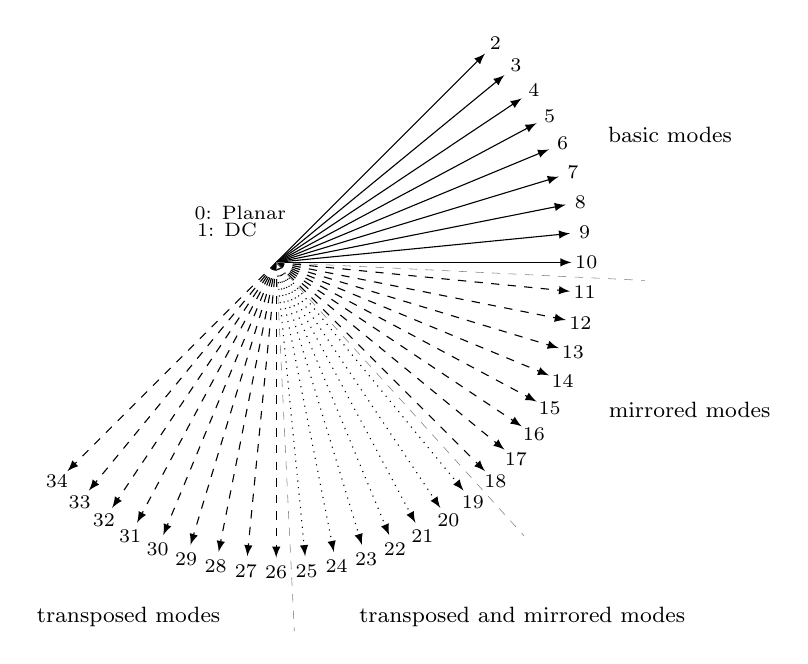
\begin{tikzpicture}[scale=1.25]

	\def\startx{0}
	\def\starty{0}
	\def\radius{3.0}
	\def\startangle{45}
	\def\colour{black}
	\def\style{}

	\draw (-0.365, 0.5) node {\scriptsize 0: \color{\colour}{Planar}};
	\draw (-0.50, 0.5) node[below] {\scriptsize 1: \color{\colour}{DC}};

	% draw the basic HEVC IPMs with different styles
	\foreach \direction in {2,3,...,34}
	{%
		% set the angle of current prediction direction 
		\pgfmathsetmacro{\angle}{\startangle - (\direction - 2) * 180 / 32}
		% \ifthenelse{\direction = 18}{\def\thickness{very thick}};
		% \ifthenelse{\direction = 26}{\def\thickness{very thick}};
		% basic modes
		\ifthenelse{\direction > 1 \AND \direction < 11}{\def\colour{black}};
		% mirror modes
		\ifthenelse{\direction > 10 \AND \direction < 19}{\def\style{dashed}};
		% transposed and mirrored modes
		\ifthenelse{\direction > 18 \AND \direction < 26}{\def\style{dotted}};
		% transposed modes
		\ifthenelse{\direction > 25 \AND \direction < 35}{\def\style{dashed}};
		% draw the directions
		\draw[-latex,\colour, \style] (\startx,\starty) --++ (\angle:\radius);
		% label each prediction direction
		\draw(\angle:\radius + 0.15) node {\scriptsize \direction};
	}

	% draw separators
	\foreach \direction in {10, 18, 25}
	{
		\pgfmathsetmacro{\angle}{\startangle - (\direction + 0.5 - 2) * 180 / 32}
		\draw[help lines, dashed] (\startx,\starty) --++ (\angle:\radius + 0.75);
	}

	% label IPM groups
	\draw (4,1.3) node {\footnotesize basic modes};
	\draw (4.2,-1.5) node {\footnotesize mirrored modes};
	\draw (2.5,-3.6) node {\footnotesize transposed and mirrored modes};
	\draw (-1.5,-3.6) node {\footnotesize transposed modes};

\end{tikzpicture}

% vim:set filetype=tex:

		\end{block}
	\end{minipage}
	\hfill
	\begin{minipage}{0.48\textwidth}
		\begin{block}{Operations applied to blocks}
			$$\X =
			\begin{cases}
				\A \, \x & \;\;\, 0 \le \text{IPM} \le 10 \\
				\A \, \curvearrowupdown\x & 11 \le \text{IPM} \le 18 \\
				\A \, \curvearrowupdown\x^T & 19 \le \text{IPM} \le 25 \\
				\A \, \x^T & 26 \le \text{IPM} \le 34 \\
			\end{cases}$$
		\end{block}
		\vfill$\,$
	\end{minipage}
\end{frame}

\subsubsection{Results on the ROM --- BD-rate plane}

\begin{frame}{\currentname}

	\only<1>{\definecolor{greenish}{RGB}{0,145,0}
\begin{tikzpicture}
	\pgfplotsset{/tikz/font={\tiny}}
	\begin{axis}[
			% title=Bitrate savings: $-8.94\%$. SNR improvement: $0.46$ dB,
			xlabel={ROM (kB)},
			ylabel={Y BD-rate (\%)},
			grid=both,
			scale only axis,
			width=0.9\textwidth,
			height=0.7\textheight,
			xtick={0.25,0.5,1,2,4,8,16,32,64,128,256,512,1024},
			xticklabels={0.25,0.5,1,2,4,8,16,32,64,128,256,512,1024},
			% x tick label style={
			% 	/pgf/number format/.cd,
			% 	fixed,
			% 	fixed zerofill,
			% 	precision=0,
			% },
			% scaled x ticks=false,
			ytick={0,-0.5,...,-4},
			y tick label style={
				/pgf/number format/.cd,
				fixed,
				fixed zerofill,
				precision=1,
				/tikz/.cd
			},
			xmode=log,
			log basis x=2,
			xmin=0.5, xmax=1024,
			ymin=-4.0, ymax=0,
			legend style={nodes=right},
			legend pos= south west
		]

		\addlegendentry{$4\times4$ hom. MDTC}
		\addplot [mark=* ,mark size=1pt, red, thick, dashed,
		visualization depends on=\thisrow{alignment} \as \alignment,
		nodes near coords, % Place nodes near each coordinate
		point meta=explicit symbolic, % The meta data used in the nodes is not explicitly provided and not numeric
		every node near coord/.style={anchor=\alignment} % Align each coordinate at the anchor 40 degrees clockwise from the right edge
		] table [meta index=2] {
		rom	dtt_bdrate	dtt_label	alignment
		1.64	-0.49	\tiny{\color{black}4s1--8s0}	-90
		3.28	-0.67	\tiny{\color{black}4s2--8s0}	-90
		6.56	-0.82	\tiny{\color{black}4s4--8s0}	-90
		13.13	-0.93	\tiny{\color{black}4s8--8s0}	-90
		26.25	-0.98	\tiny{\color{black}4s16--8s0}	-90
		52.2	-1.01	\tiny{\color{black}4s32--8s0}	-90
		};

		% \addlegendentry{$8\times8$ hom. MDTC}
		% \addplot [mark=*, mark size=1pt, blue, thick, dashed,
		% visualization depends on=\thisrow{alignment} \as \alignment,
		% nodes near coords, % Place nodes near each coordinate
		% point meta=explicit symbolic, % The meta data used in the nodes is not explicitly provided and not numeric
		% every node near coord/.style={anchor=\alignment} % Align each coordinate at the anchor 40 degrees clockwise from the right edge
		% ] table [meta index=2] {
		% rom	dtt_bdrate	dtt_label	alignment
		% 6.56	-0.84	\tiny{\color{black}4s0--8s1}	90
		% 13.13	-1.33	\tiny{\color{black}4s0--8s2}	225
		% 26.25	-1.72	\tiny{\color{black}4s0--8s4}	225
		% 52.50	-2.10	\tiny{\color{black}4s0--8s8}	225
		% 105.00	-2.48	\tiny{\color{black}4s0--8s16}	225
		% 210.00	-2.79	\tiny{\color{black}4s0--8s32}	225
		% 420.00	-3.07	\tiny{\color{black}4s0--8s64}	225
		% 840.00	-3.33	\tiny{\color{black}4s0--8s128}	45
		% };

		% \addlegendentry{Comb. hom. MDTC}
		% \addplot [mark=*, mark size=1pt, greenish, thick, dashed,
		% visualization depends on=\thisrow{alignment} \as \alignment,
		% nodes near coords, % Place nodes near each coordinate
		% point meta=explicit symbolic, % The meta data used in the nodes is not explicitly provided and not numeric
		% every node near coord/.style={anchor=\alignment} % Align each coordinate at the anchor 40 degrees clockwise from the right edge
		% ] table [meta index=2] {
		% rom	dtt_bdrate	dtt_label	alignment
		% 8.20	-1.38	\tiny{\color{black}4s1--8s1}	180
		% 14.77	-1.80	\tiny{\color{black}4s1--8s2}	180
		% 16.41	-1.97	\tiny{\color{black}4s2--8s2}	180
		% 27.89	-2.14	\tiny{\color{black}4s1--8s4}	180
		% 32.81	-2.45	\tiny{\color{black}4s4--8s4}	180
		% 59.06	-2.76	\tiny{\color{black}4s4--8s8}	180
		% 65.62	-2.83	\tiny{\color{black}4s8--8s8}	180
		% 118.12	-3.15	\tiny{\color{black}4s8--8s16}	180
		% 223.12	-3.39	\tiny{\color{black}4s8--8s32}	-90
		% 236.25	-3.44	\tiny{\color{black}4s16--8s32}	90
		% };

		% \addlegendentry{$4\times4$ iterations}
		% \pgfplotstableread{figures/vmdtc_iter_4.dat}\table
		% \addplot[red, thick, mark=*, mark size=0.5pt, smooth]
		% table[x=rom,y=bdrate,col sep=tab] from \table;

		% \addlegendentry{$8\times8$ iterations}
		% \pgfplotstableread{figures/vmdtc_iter_8.dat}\table
		% \addplot[blue, thick, mark=*, mark size=0.5pt, smooth]
		% table[x=rom,y=bdrate,col sep=tab] from \table;

		% \addlegendentry{Comb. het. MDTC}
		% \addplot [mark=*, mark size=1pt, greenish, thick,
		% visualization depends on=\thisrow{alignment} \as \alignment,
		% nodes near coords, % Place nodes near each coordinate
		% point meta=explicit symbolic, % The meta data used in the nodes is not explicitly provided and not numeric
		% every node near coord/.style={anchor=\alignment} % Align each coordinate at the anchor 40 degrees clockwise from the right edge
		% ] table [meta index=2] {
		% rom	dtt_bdrate	dtt_label	alignment
		% 0.98	-0.74	 \tiny{\color{black}1 kB}	0
		% 1.97	-1.02	 \tiny{\color{black}2 kB}	0
		% 3.98	-1.39	 \tiny{\color{black}4 kB}	0
		% 7.97	-1.82	 \tiny{\color{black}8 kB}	0
		% 12.00	-2.10	 \tiny{\color{black}12 kB}	0
		% 15.61	-2.22	 \tiny{\color{black}16 kB}	0
		% 23.95	-2.52	 \tiny{\color{black}24 kB}	0
		% 31.78	-2.68	 \tiny{\color{black}32 kB}	0
		% 47.39	-2.85	 \tiny{\color{black}48 kB}	0
		% 63.89	-3.00	 \tiny{\color{black}64 kB}	0
		% 95.53	-3.27	 \tiny{\color{black}96 kB}	0
		% 127.41	-3.41	 \tiny{\color{black}128 kB}	0
		% };

\end{axis}
\end{tikzpicture}
}
	\only<2>{\input{./figures/vmdtc_iter_plot_2.tex}}
	\only<3>{\input{./figures/vmdtc_iter_plot_3.tex}}
	\only<4>{\input{./figures/vmdtc_iter_plot_4.tex}}
	
\end{frame}

\begin{frame}{Summary and conclusions}
	\begin{block}{Systems on demand (performances on the HEVC test set)}
		\vspace{1em}
		\centering
		\begin{tabular}{l|r|r|r|r}
			System
			& \multicolumn{1}{c|}{16 kB}
			& \multicolumn{1}{c|}{32 kB}
			& \multicolumn{1}{c|}{64 kB}
			& \multicolumn{1}{c}{128 kB} \\
			\hline\hline
			Y BD-rate & -2.87\%  & -3.21\%  & -3.55\%  & -3.79\%\\
			Encoding  & 372\%    & 481\%    & 761\%    & 1297\%\\
			Decoding  & 105\%    & 105\%    & 105\%    & 105\%\\
			% ROM       & 15.84 kB & 31.92 kB & 63.84 kB & 123.38 kB\\
		\end{tabular}
	\end{block}
	\begin{block}{Remarkable points}
		\begin{itemize}
			\item ROM can be reduced up to a third of its original value
			\item Bit-rate savings are maintained
			\item Coding complexity remains more or less untouched
		\end{itemize}
	\end{block}
\end{frame}

\subsection{MDTC systems based on Discrete Trigonometric Transforms}

\begin{frame}{Discrete Trigonometric Transforms (DTTs)}
\framesubtitle{DCTs and DSTs}
\begin{block}{DTT strengths}
	\begin{itemize}
		\item Fast algorithms
			\begin{itemize}
				\item number of operations in the order of $N\log_2 N$ instead
					of $N^2$
			\end{itemize}
		\item Transform coefficients can be computed analytically
			\begin{itemize}
				\item notable reduction in storage requirements
			\end{itemize}
		\item They can be more easily pushed into a standard
	\end{itemize}
\end{block}
\end{frame}

\begin{frame}{Examples of $4\times4$ DTTs}
	
\begin{figure}[tb]
	\centering
	\subfloat[\bf DCT-II --- DCT-II]
	{\includegraphics[width=0.20\linewidth]
	{./figures/dtts_4/dtt_017_DCT_IIxDCT_II.png}}
	\hfill
	\subfloat[\bf DST-VII --- DST-VII]
	{\includegraphics[width=0.20\linewidth]
	{./figures/dtts_4/dtt_238_DST_VIIxDST_VII.png}}
	\hfill
	\subfloat[DCT-IV --- DCT-IV]
	{\includegraphics[width=0.20\linewidth]
	{./figures/dtts_4/dtt_051_DCT_IVxDCT_IV.png}}
	\hfill
	\subfloat[DCT-III --- DCT-IV]
	{\includegraphics[width=0.20\linewidth]
	{./figures/dtts_4/dtt_035_DCT_IIIxDCT_IV.png}}

	\subfloat[DST-VII --- DCT-IV]
	{\includegraphics[width=0.20\linewidth]
	{./figures/dtts_4/dtt_227_DST_VIIxDCT_IV.png}}
	\hfill
	\subfloat[DST-V --- DCT-IV]
	{\includegraphics[width=0.20\linewidth]
	{./figures/dtts_4/dtt_067_DCT_VxDCT_IV.png}}
	\hfill
	\subfloat[DST-VII --- DCT-V]
	{\includegraphics[width=0.20\linewidth]
	{./figures/dtts_4/dtt_228_DST_VIIxDCT_V.png}}
	\hfill
	\subfloat[DST-VII --- DST-II]
	{\includegraphics[width=0.20\linewidth]
	{./figures/dtts_4/dtt_105_DCT_VIIxDST_II.png}}

	% \caption{$4\times4$ DTT combination examples}
	% \label{fig:some_dtts}
\end{figure}
\end{frame}

\begin{frame}{Designing a DTT-based MDTC system}
	\begin{block}{Using the RDOT metric to classify}
		\begin{itemize}
			\item Transforms are already known (8 DCTs, 8 DSTs and their
				inverses)
			\item There are 256 possible transforms
			% \item Combining horizontal and vertical transforms with geometrical pre-processing:
			% 	\begin{itemize}
			% 		\item 2048 combinations
			% 		\item 256 combinations allowing a scanning after transforms
			% 	\end{itemize}
			\item Complexity of the classifying algorithm:
				\begin{itemize}
					\item selection the best combination of $N$ transforms
						amongst 256
					\item example for $N=4$:
						\vspace{-0.5em}
						\begin{align}
							\begin{pmatrix}
								256 \\
								4
							\end{pmatrix} =
							\num{174792640}\approx\num{1.75e8}
						\end{align}
				\end{itemize}
			\item The algorithm suboptimality increases with $N$
			\item Symmetries and non-homogeneous repartition of transforms are
				used with DTTs
		\end{itemize}
	\end{block}
\end{frame}

\begin{frame}{Performances of DTT-based MDTC systems}
	\only<1>{\input{./figures/vmdtc_iter_plot_4.tex}}
	\only<2>{\input{./figures/vmdtc_iter_plot_5.tex}}
\end{frame}

\begin{frame}{Summary}
	\begin{block}{DTT-based MDTC system compared to RDOT-based ones}
		\vspace{1em}
		\begin{tabular}{l|r|r|r||r|r|r}
			& \multicolumn{3}{c||}{DTT} & \multicolumn{3}{c}{RDOT}\\
			System
			% \multirow{2}{2cm}{\diagbox{System}{Measure}}
			& \multicolumn{1}{c|}{1 kB}
			& \multicolumn{1}{c|}{2 kB}
			& \multicolumn{1}{c||}{4 kB}
			& \multicolumn{1}{c|}{1 kB}
			& \multicolumn{1}{c|}{2 kB}
			& \multicolumn{1}{c}{4 kB} \\
			\hline\hline
			Y BD-rate & -1.28\% & -1.54\% & -1.86\% & -0.89\% & -1.25\% & -1.71\% \\
			Encoding  &   164\% &   177\% &   230\% &   126\% &   150\% &   175\% \\
			Decoding  &   100\% &   100\% &   100\% &   105\% &   105\% &   105\% \\
		\end{tabular}
	\end{block}
	\begin{block}{Remarkable points}
		\begin{itemize}
			% \item No fast algorithms were used in this experiment
			\item Almost 2\% bit-rate savings with low complexity
			\item Performances could be higher by improving the learning
				algorithm
			\item DTTs make transforms for bigger block sizes more reasonable
				\begin{itemize}
					\item room for improvement when using $16\times16$ or even
						$32\times32$ transforms
				\end{itemize}
		\end{itemize}
	\end{block}
\end{frame}

\section{Conclusions}

\subsection*{Conclusions}

\begin{frame}{\currentname}
	\begin{block}{Interest of multiple transforms for video coding}
		\begin{itemize}
			% \item Several working solutions have been implemented providing
			% 	significant bit-rate savings over HEVC
			\item This technique alone is able to achieve significant bit-rate
				savings over HEVC, depending on complexity:
				\begin{itemize}
					\item non-separable transforms: up to 7\%
					\item separable transforms: up to 4\%
					\item DTTs: 2\% (in progress)
					\item reminder: HEVC improves intra coding by 22\% over
						AVC
				\end{itemize}
			\item Systematic on demand design with the RDOT metric
				\begin{itemize}
					\item the $\ell_0$ has proved to be a robust rate
						approximation
					\item independence from residuals PDF has been proved
				\end{itemize}
		\end{itemize}
	\end{block}
\end{frame}

\subsection*{Perspectives and future work}

\begin{frame}{\currentname}
	\begin{block}{Immediate action points}
		\begin{itemize}
			\item extend the system
				\begin{itemize}
					\item bigger TU sizes
					\item inter coding (gain in RA is about 2/3 of AI)
					\item chroma
				\end{itemize}
			\item coding complexity
				\begin{itemize}
					\item incomplete transforms
					\item exhaustive search might not be necessary
				\end{itemize}
			\item transform signalling and quantisation
		\end{itemize}
	\end{block}
	\begin{block}{Multiple transforms in future video formats}
		\begin{itemize}
			\item Multiple transforms are part of the preliminary draft for a
				future video coder by ITU and MPEG
		\end{itemize}
	\end{block}
\end{frame}

\begin{frame}{Publications}
	\begin{block}{Conference papers}
		\begin{itemize}
			\item 2 VCIP 2014 presented papers
			\item 2 ICIP 2015 presented papers
			\item 1 ICASSP 2016 submitted paper
		\end{itemize}
	\end{block}
	\begin{block}{Patents}
		\begin{itemize}
			\item 5 filled patent applications
		\end{itemize}
	\end{block}
\end{frame}

\usebackgroundtemplate{%
\begin{tikzpicture}[remember picture, overlay]%
	\node at (current page.center) {
\includegraphics[width=0.9\paperwidth]{background}};%
\end{tikzpicture}}

\begin{frame}
	\Huge
	Thank you for your attention
	\definecolor{protonblue}{RGB}{102,102,153}
	\vspace{1em}
	\Large
	Questions?
	\vspace{0.75cm}
	\thispagestyle{empty}
	\vfill
	\begin{flushright}
		\normalsize
		Adrià Arrufat
		\footnotesize{%
			\bf \color{protonblue}\href{mailto:adria.arrufat@protonmail.ch}
			{\texttt{adria.arrufat@protonmail.ch}}}
	\end{flushright}
\end{frame}

\usebackgroundtemplate{}

\end{document}
